%% This is an example first chapter.  You should put chapter/appendix that you
%% write into a separate file, and add a line \include{yourfilename} to
%% main.tex, where `yourfilename.tex' is the name of the chapter/appendix file.
%% You can process specific files by typing their names in at the 
%% \files=
%% prompt when you run the file main.tex through LaTeX.
\chapter{Methodology}

In this chapter, an introduction to machine learning methods is presented. 
Machine learning methods is discussed with a focus on applications.
Finally, a supervised learning method, Support Vector Machines (SVM) is explained since it is the method used for classification in this thesis.

\section{Machine Learning}

The aim of machine learning methods is to train a model with a given data set in order to predict the output values corresponding to a new input. 
According to Arthur Samuel, who coined the term machine learning, "Machine learning is the field of study that gives computers the ability to learn without being explicitly programmed". 
Another definition offered by Tom Mitchell in 1998, quite new compared to to the one by Samuel in 1959, is stated as: "A computer program is said to learn from experience E with respect to some task T and some performance measure P, if its performance on T, as measured by P, improves with experience E".

\subsection{Introduction}
Machine learning methods are mainly handled under two main categories: supervised and unsupervised learning as shown in Fig.~\ref{fig:machineLearningMethodsSerious}. 

\begin{figure}
\begin{center}
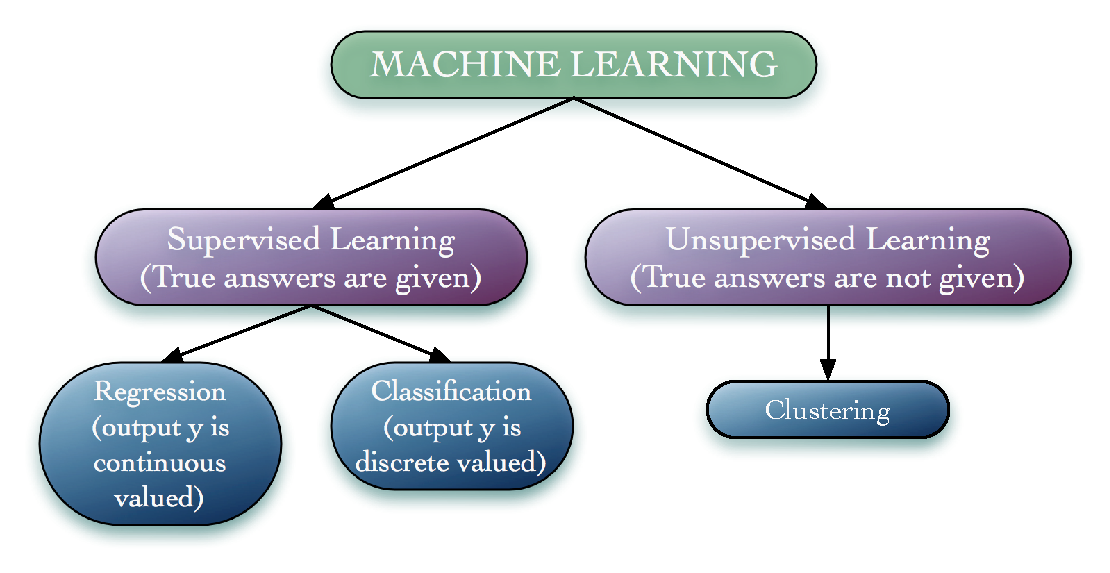
\includegraphics[width=14cm]{figures/machineLearningMethodsSerious}    % The printed column width is 8.4 cm.
\caption{Common machine learning methodologies} 
\label{fig:machineLearningMethodsSerious}
\end{center}
\end{figure}

In supervised learning, \textit{"right answers"} are available for each training input in the data set.
Supervised learning methods are comprised of two phases, the learning and the prediction as shown in Fig.~\ref{fig:supervisedLearningBasics}.
The first phase is comprised of learning from the available data to understand how the system behaves. 
In the second phase, the idea is to predict what will be the output of the system for a given input, depending on the knowledge about the system that you gained via the learning phase. 

\begin{figure}
\begin{center}
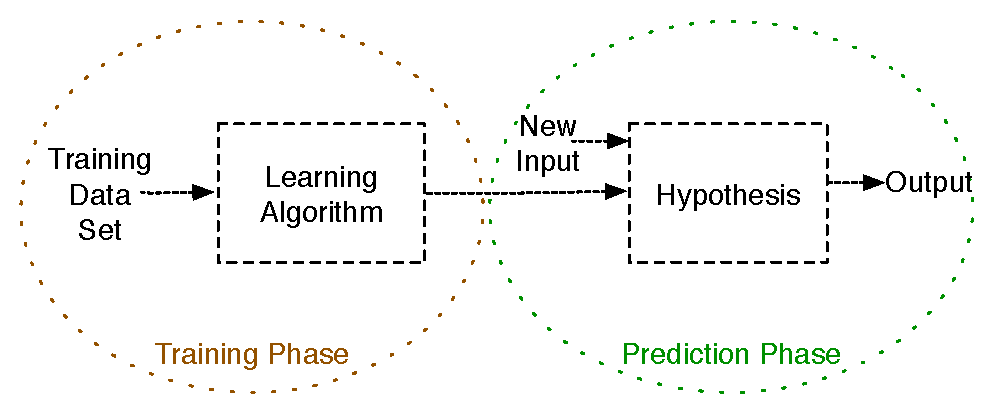
\includegraphics[width=14cm]{figures/supervisedLearningBasics}    % The printed column width is 8.4 cm.
% For the old picture 
% \includegraphics[width=12cm]{figures/machineLearningBasics}   
\caption{Supervised learning basics } 
\label{fig:supervisedLearningBasics}
\end{center}
\end{figure}
 
The most common types of supervised leaning are the regression and classification problems. 
Since these are both supervised learning types, the \textit{"right answer"} (right values of the output $y$) for each example is assumed to be known. 

In unsupervised learning, the \textit{"right answers"} corresponding to the training input are not available. 
There are other machine learning algorithms, such as those for reinforcement learning, which combine supervised and unsupervised learning. 

\subsection{Terminology}

A basic introduction to frequently used terms in machine learning is given in this section.  
Table~\ref{arm:machineLearningTerminology} shows representations of commonly used variables in machine learning. 
Although representations could differ from one reference to the other, throughout this thesis, one coherent representation given in Table~\ref{arm:machineLearningTerminology} is followed. 

\begin{table}
\caption{Machine learning terminology}
\label{arm:machineLearningTerminology}
\begin{center}
\begin{tabular}{||l|l||}\hline
x & input variable or feature \\\hline
y & output variable or target variable \\\hline
\textbf{X} & input variable vector or feature vector \\\hline
\textbf{y} & output variable vector or target variable vector \\\hline
m & number of training examples \\\hline
n & number of features \\\hline
i & index of training examples \\\hline
j & index of features \\\hline
$\textbf{x}_j^{(i)}$ & $i^{th}$ training example for feature $j$ \\\hline
$\textbf{y}^{(i)}$ & $i^{th}$ training output  \\\hline
$\textbf{h}_{\bm{\theta}}(\textbf{x})$ &hypothesis function (model)\\\hline
$\bm{\theta}$ &parameter set\\\hline
$\textbf{J}({\bm{\theta}})$ &cost function  \\\hline

\end{tabular}
\end{center}
\end{table}

Many of the machine learning tools, such as \emph{MATLAB Statistics and Machine Learning Toolbox} or \emph{Tensorflow}, have default settings and are easy to used for beginners. 
Although they would most probably not achieve optimized results, which would be the case in the hands of an experienced user, a beginner can easily start using those tools by sending input and output vectors as arguments to the machine learning functions. 

The configurations of input and output vectors to feed the learning algorithms might change from one to the other, but there is still a common convention that would be compatible with many. 
In this representation, each instance is given in different rows of the input vector. 
An example of predicting housing prices taken from Ref.~\cite{andrewNgMachLearning} is given to show the way to constitute the input and output matrix. 
Table~\ref{arm:exampHousingPrices} uses a supervised learning regression example to show input and output vector representations. 
The aim of the problem in this example is to predict prices of houses given the surface area. 
For that, known examples of houses with surface area and corresponding price are given. 
Since the aim of the problem is to predict the price of a house given the surface area, the price of house is the output of the problem. 
To predict the price, the available information that is known to effect the price of a house is the surface area of the house, making it the input variable. 
So, in Table~\ref{arm:exampHousingPrices} each row corresponds to a different house, second column (surface area of house) constitute the input vector and the last row (price in \$1000s) corresponds to the output vector. 

\begin{table}
\caption{Training set $(\textbf{x},\textbf{y})$ of housing prices - one-feature example}
\label{arm:exampHousingPrices}
\begin{center}
\begin{tabular}{ || c | c | c ||}\hline
\textbf{training example index} $(i)$ & \textbf{Size in $feet^2$} ($\textbf{x}$) & \textbf{Price in $1000 \$ s$} ($\textbf{y}$) \\\hline
1 & 2104	   & 460 \\\hline
2 & 1416	   & 232 \\\hline
3 & 1534	   & 315 \\\hline
4 & 852	   & 178 \\\hline
$\vdots$ & $x^{(i)}$   & $y^{(i)}$ \\\hline
m & $x^{(m)}$   & $y^{(m)}$ \\\hline
\end{tabular}
\end{center}
\end{table}

In this problem, there is an assumption that the price of a house is only dependent on the surface area which would not hold in the real case. 
In real problems, it is more common that the output would depend not only on one variable but more. 
For that reason, the input vector in a realistic example would rather be an input matrix having different features in its columns as given in Table~\ref{arm:exampleMultiFeatures}. 
Here, in this example, the output is still the price of the house, but now the features which correspond to each column of an input matrix (or sometimes called the feature matrix) are the surface area, the number of bedrooms, and can be enlarged up to a chosen number of features. 
It should be kept in mind that the selection of features that would lead to a better prediction of the output is a challenging problem and usually requires experience on the system of interest. 

\begin{table}
\caption{Training set $(\textbf{x},\textbf{y})$ of housing prices - multi-feature example}
\label{arm:exampleMultiFeatures}
\begin{center}
\begin{tabular}{ ||p{2cm}|p{2cm}|p{2cm}|p{2cm}|p{2cm}|p{2cm}||}\hline
\textbf{training example index} $(i)$ & \textbf{Size in $feet^2$} ($\textbf{x}_1^{(i)}$) & \textbf{Number of bedrooms} ($\textbf{x}_2^{(i)}$) & \textbf{Feature j} ($\textbf{x}_j^{(i)}$) & \textbf{Feature n} ($\textbf{x}_n^{(i)}$) &\textbf{Price in $1000 \$ s$} ($\textbf{y}$) \\\hline
1 & 2104	& 5  & $\textbf{x}_j^{(1)}$ & $\textbf{x}_n^{(1)}$ & 460 \\\hline
2 & 1416 & 3 & $\textbf{x}_j^{(2)}$ & $\textbf{x}_n^{(2)}$ & 232 \\\hline
3 & 1534 & 3 & $\textbf{x}_j^{(3)}$ & $\textbf{x}_n^{(3)}$ & 315 \\\hline
4 & 852 & 2 & $\textbf{x}_j^{(4)}$ & $\textbf{x}_n^{(4)}$ & 178 \\\hline
$\vdots$ & $\textbf{x}_1^{(i)}$  & $\textbf{x}_2^{(i)}$  & $\textbf{x}_j^{(i)}$   & $\textbf{x}_n^{(i)}$ & $\textbf{y}^{(i)}$ \\\hline
m & $\textbf{x}_1^{(m)}$  & $\textbf{x}_2^{(m)}$  & $\textbf{x}_2j^{(m)}$   & $\textbf{x}_n^{(m)}$ & $\textbf{y}^{(m)}$ \\\hline
\end{tabular}
\end{center}
\end{table}


%\clearpage
%\newpage


\subsection{Steps towards the learning machine}

\subsubsection{Visualizing the data}

Having a preliminary glance at data, might give the designer an idea about the ways to tackle the problem since it is the designer who selects the features, the model, and the type of cost function. 
It is true that the algorithms are optimizing some parameters of the model and the cost function but still the structure itself is usually supplied by a human. 
%Although there are tricks to select those in a better sense, machines still have a way to go towards Skynet\footnote{From movie Terminator: ``Skynet is a fictional neural net-based conscious group mind and artificial general intelligence (see also superintelligence) system that features centrally in the Terminator franchise and serves as the franchise's true main antagonist.''}.

Fig.~\ref{fig:housingPrices} shows the housing price depending on the surface area corresponding to the data given in Table~\ref{arm:exampHousingPrices}.
In this example, house prices are the output (target) variable given in y-axis and size (surface area in $feet^2$) is the feature (input) variable given in x-axis. 
Since output y is the price which is a continuous value (thus not a label representing a class), this problem is called a regression problem. Plotting the given data, shows that the problem could be modeled by a linear model (a linear line to fit the data given). Then, linear regression can be applied.

\begin{figure}
\begin{center}
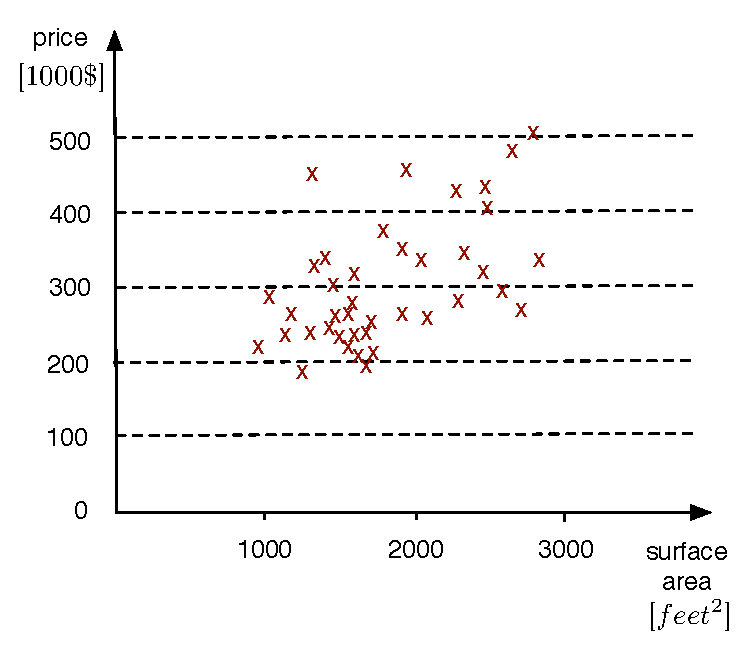
\includegraphics[width=11cm]{figures/linearRegressionExamp}    % The printed column width is 8.4 cm.
\caption{Regression example - Housing prices as a function of surface area of the house \cite{andrewNg_MachLearning}} 
\label{fig:housingPrices}
\end{center}
\end{figure}

\begin{figure}
\begin{center}
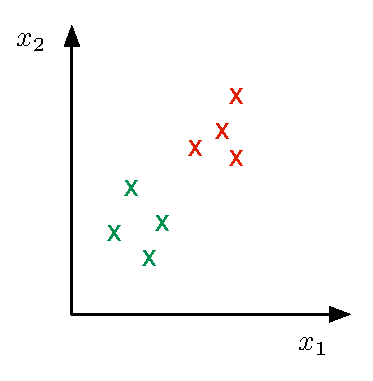
\includegraphics[width=5cm]{figures/classificationEx2}    % The printed column width is 8.4 cm.
\caption{Classification example} 
\label{fig:classificationEx2}
\end{center}
\end{figure}

Since an example of a regression problem has been given above, a preliminary look at a classification problem is presented as follows. 
Fig.~\ref{fig:classificationEx2} presents a classification problem since the aim is to distinguish the class that a new input instance will belong to. 
Here, the vertical dimension is not the output as in the previous example of linear regression but is another feature ($x_2$ in this example). 

The information about the output is represented with the colors of the samples in the feature space.
Fig.~\ref{fig:classificationEx1} shows the output vs. inputs of a classification problem. 
This is just to show the difference between regression and classification problem figures. 
Usually in regression problems the y-axis represents the output. 
Here, there is a direct analogy by representing a classification problem as a regression problem, the x-axis representing the input and the y-axis representing the output. 
But usually in classification problems, the value of y (which class it corresponds to) is represented with discrete values representing the different classes as shown in Fig.~\ref{fig:classificationEx2}.

By just plotting the samples, in this example, it seems that logistic regression could yield satisfactory results since the data seems to be separated by a linear decision boundary. 
A decision boundary is a curve that separates the training data examples which belongs to different classes. 

It is possible to choose the model structure that would represent the problem satisfactorily via visualizing the data set when the number of features is not large.
With an increasing number of features, determining the degree of the polynomial via visualizing the data to represent the input output relationship could be more complicated. 
In that case, the user should refer to model selection techniques rather than the insights gained by data visualization. 

\begin{figure}
\begin{center}
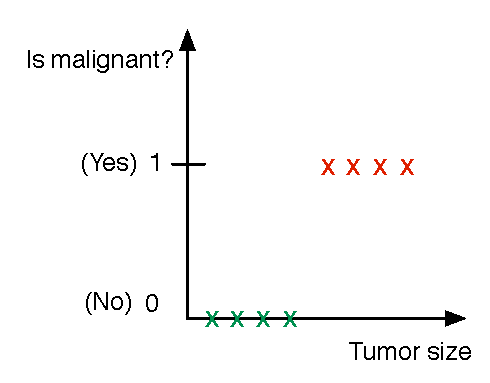
\includegraphics[width=7cm]{figures/classificationEx1}    % The printed column width is 8.4 cm.
\caption{Classification example - output vs input} 
\label{fig:classificationEx1}
\end{center}
\end{figure}


\subsubsection{Feature Mapping}

Depending on the results from visualizing data, it might be necessary to map the features since a straightforward implementation of linear / logistic regression might result in linear model, linear decision boundary respectively. 
So for the cases that a linear model will not be satisfactory enough to describe the training data, feature mapping should be applied.

The housing price prediction problem can be revisited here to give an example on feature mapping.
The data given in Table~\ref{arm:exampHousingPrices} and plotted in Fig.~\ref{fig:housingPrices} is a regression problem with one feature (surface area of house).
To fit more accurately to the training data given, new features can be artificially added to the system as below, where the new features will be functions of the original feature.

\begin{align}
\label{eqn:costFuncExamp1}
\begin{split}
h_{\theta}(\bm{x}) & = \theta_0 + \theta_1 x_1 + \theta_2 x_2 + \theta_3 x_3
\\
& = \theta_0 + \theta_1 (size) + \theta_2 {(size)}^2 + \theta_3 {(size)}^3
\end{split}
\end{align}

where

\begin{align}
\label{eqn:featureMapping1}
\begin{split}
x_1 & = size
\\
x_2 & = size^2
\\
x_3 & = size^3
\end{split}
\end{align}

\begin{figure}
\begin{center}
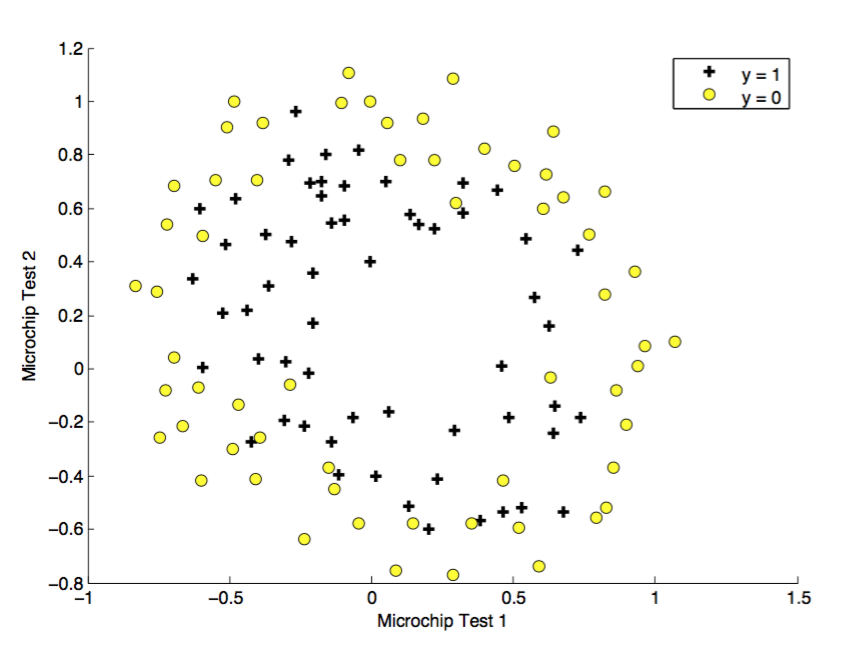
\includegraphics[width=13cm]{figures/classificationMicrochip}    % The printed column width is 8.4 cm.
\caption{Classification example - complex decision boundaries \cite{andrewNg_MachLearning}} 
\label{fig:classificationEx3}
\end{center}
\end{figure}

By changing the model via adding features, it is now possible to fit a nonlinear curve to the training data as given in Fig.~\ref{fig:underOverFit}.

Another example that requires a nonlinear model to fit the data set is the microchip assessment problem.
This example is also taken from the lecture notes of a machine learning course by Andrew Ng \cite{andrewNgMachLearning}. 
This is a two-class classification problem, where one class of microchips is faulty while the other class is functional.
It is seen from the Fig.~\ref{fig:classificationEx3} that a linear decision boundary will not appropriately serve to classify the data. 
So, in order to apply logistic regression for this problem, feature mapping is necessary. 
An example of a mapped feature vector that could give a satisfactory decision boundary to classify the two classes could be given as

\begin{equation}{\label{eqn:featureMapping2}}
\bm{x_{mapped}}
=\,
\begin{bmatrix}
1 & x_1 & x_2 & x_1^2 & x_1x_2 & x_2^2 & x_1^3 \cdots & x_1x_2^5 & x_2^6 
\end{bmatrix}
\,^ T
\end{equation} 

Mapping of the features could be done in various ways. 
Let's take another example of a binary (two-class) classification problem with 100 features, which needs a nonlinear decision boundary to achieve a satisfactory classification.
One way to map the feature set could be such that only the quadratic terms are taken into account, which would result in a new feature set such as
 
\begin{equation}{\label{eqn:featureMapping3}}
\bm{x_{mapped}}
=\,
\begin{bmatrix}
x_1^2 & x_1x_2 & x_1x_3 & \cdots & x_1x_{100} & x_2^2 & x_2x_3 & \cdots & x_3^2 & x_3x_4  \cdots  
\end{bmatrix}
\,^ T
\end{equation} 

with a complexity $O(n^2) \sim \frac{n^2}{2}$

If 3\textsuperscript{rd} order terms are considered, the new feature set becomes

\begin{equation}{\label{eqn:featureMapping4}}
\bm{x_{mapped}}
=\,
\begin{bmatrix}
x_1^3 & x_1x_2x_3 & x_1^2x_2 & \cdots  & x_{11}x_{13}x_{17} & \cdots  
\end{bmatrix}
\,^ T
\end{equation} 

\begin{figure}
\begin{center}
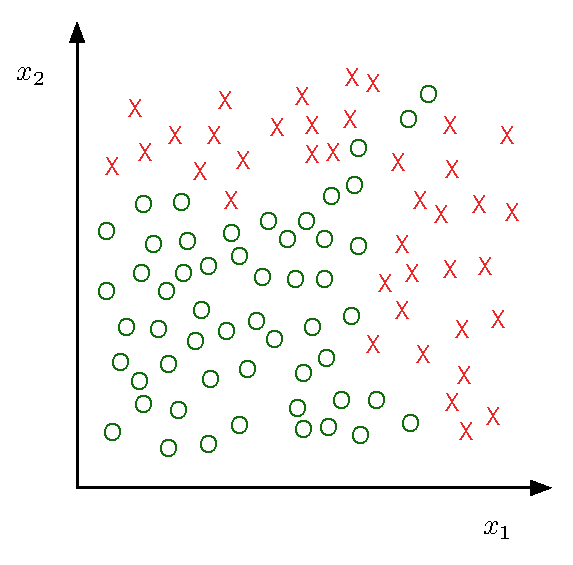
\includegraphics[width=6cm]{figures/complexDecisionBoundary}    % The printed column width is 8.4 cm.
\caption{Classification example - complex decision boundaries} 
\label{fig:complexBoundary}
\end{center}
\end{figure}

\begin{figure}
\begin{center}
\includegraphics[width=14.1cm]{figures/ml_followChart}    % The printed column width is 8.4 cm.
\caption{Simplified guide for feature mapping} 
\label{fig:ml_followChart}
\end{center}
\end{figure}


It is important to point out that, with a higher dimensional feature vector, the model will tend to fit more accurately to the training set but might generalize more poorly to new input. 
This is called overfitting which is a common problem for many machine learning applications. 
More explanations about overfitting and ways to overcome it will be explained in the regularization section. 
Increasing the dimensionality of the features, the model might become more computationally expensive as well.

To fit a model or decision boundary of a circular or elliptical shape, only a subset of features can be considered such as

\begin{equation}{\label{eqn:featureMappin54}}
\bm{x_{mapped}}
=\,
\begin{bmatrix}
x_1^2 & x_2^2 & x_3^2 & \cdots & x_N^2  
\end{bmatrix}
\,^ T
\end{equation} 

Finally, when the number of features are small, but it can not fit complex models or boundaries such as in Fig.~\ref{fig:complexBoundary}, then the addition of higher terms such as those given in 
Equ.~\ref{eqn:featureMapping3} or the use of Neural Networks should be considered.
A scheme to help select the strategy for mapping is given in  Fig.~\ref{fig:ml_followChart}. 

\subsubsection{Vectorized form of the problem}

The model can be written in a vectorized form to accommodate the larger number of features in a more compact form.
To write in compact form, an extra feature $\bm{x}_0 = 1$ is added to the feature vector such as

\begin{equation}{\label{eqn:featureVector}}
\bm{x}
=\,
\begin{bmatrix}
x_0 \quad x_1 \quad x_2 \quad \cdots \quad x_n 
\end{bmatrix}
^T
\end{equation} 

 Fig.~\ref{fig:addArtificialFeature} shows the addition of the artificial feature in the feature matrix.

\begin{figure}
\begin{center}
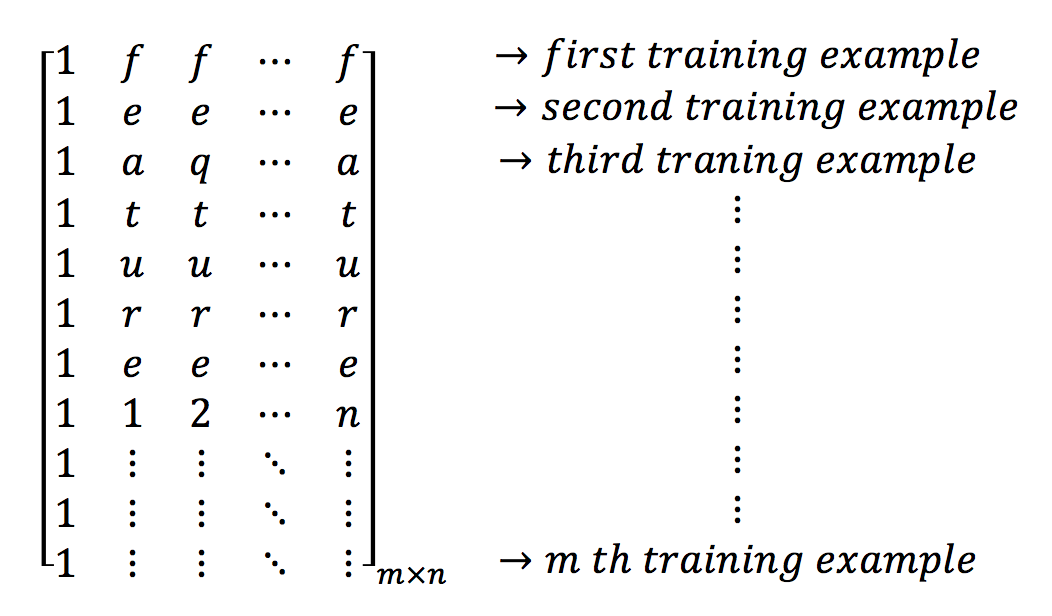
\includegraphics[width=9cm]{figures/addArtificialFeature}    % The printed column width is 8.4 cm.
\caption{Adding an artificial feature of 1s.} 
\label{fig:addArtificialFeature}
\end{center}
\end{figure}

Also parameters of the model are given in vectorial form such as

\begin{equation}{\label{eqn:parameterVector}}
\bm{\theta}
=\,
\begin{bmatrix}
\theta_0\quad \theta_1 \quad  \theta_2 \quad \cdots \quad \theta_n 
\end{bmatrix}
^T
\end{equation} 

So, for the linear regression problem with a single feature, the model is given as

\begin{equation}{\label{eqn:costFuncOneFeature}}
h_{{\bm{\theta}}}(x) = \theta_0 + \theta_1 x_1
\end{equation} 

and the model for $n$ features

\begin{equation}{\label{eqn:costFuncMltplFeature}}
h_{{\bm{\theta}}}(x) = \theta_0 + \theta_1 x_1 + \theta_2 x_2 + \cdots+ \theta_n x_n
\end{equation}

Introducing the vectorial forms of $\bm{x}$ and $\bm{\theta}$ enables the model to be written in a compact generic form such as 

\begin{equation}{\label{eqn:costFuncMltplFeature}}
h_{{\bm{\theta}}}(x) = {\bm{\theta}}^\intercal \bm{x}
\end{equation}

\subsubsection{Cost Function}

To calculate $\bm{\theta}$ that will fit a better model to the training data, optimization algorithms are used to minimize the cost function $J({\bm{\theta}})$.
Usually, the cost function and its gradient are given to the optimization algorithm as an input. 
Here, widely used cost functions for linear regression (regression problem) and logistic regression (classification problem) are given. 

The cost function for linear regression can be given as

\begin{equation}{\label{eqn:costFuncLinearRegression}}
J({\bm{\theta}})
=\,
\frac{1}{2m} \sum\limits_{i=1}^{m} \Big(h_{\bm{\theta}}(x^{(i)}) - (y^{(i)})\Big)^2  
\end{equation} 

and the cost function for logistic regression (classification) is given for a two-class classification problem (e.g $y \in \{0,1\}$) as 

\begin{equation}{\label{eqn:costFuncLogisticRegression}}
J({\bm{\theta}})
=\,
\frac{1}{m} \sum\limits_{i=1}^{m} \Big[-y^{(i)}log(h_{\bm{\theta}}(x^{(i)})) - (1-(y^{(i)}))log(1-h_{\bm{\theta}}(x^{(i)}))\Big]
\end{equation} 


\subsubsection{Selecting the model}

With a larger set of features, it might be difficult to have a sense of which model would be a better fit to the problem. 
In these cases, model selection techniques could be applied to decide which model will yield the better accuracy.

To explain the procedure, first assume a model structure is already selected or given. 
In such a problem, during training, training data is used to calculate the best model parameter vector $\bm{\theta}$ that would minimize the objective function, $J_{tranining}(\bm{\theta)}$.
%Then, the trained model is assessed with a new data set $J_{test}$, since the evaluation would be biased in favor of the training data that the model is trained for. 
%That could lead to an optimistic view of the abilities of the learning algorithm. 
The trained model is then assessed with a new independent data set $J_{test}$ to evaluate the overfitting biases favoring the training data and avoid an over-optimistic view of the abilities of the learning algorithm. 



In the model selection technique, each model is represented by a number $d$ as shown below.

\begin{alignat*}{6}
\label{eqn:exampCostFunc}
d &= 1, \quad h_{{\bm{\theta}}}(x) \ && = \theta_0 + \theta_1 x\ \ && \longrightarrow \theta^{(1)}\ \ && \quad \longrightarrow J_{cv}(\theta^{(1)})\
\\
d &= 2, \quad h_{{\bm{\theta}}}(x) \ && = \theta_0 + \theta_1 x + \theta_2 x^2 \ \ && \longrightarrow \theta^{(2)}\ \ && \quad \longrightarrow J_{cv}(\theta^{(2)})\
\\
d &= 3, \quad h_{{\bm{\theta}}}(x) \ && = \theta_0 + \theta_1 x + \theta_2 x^2 + \theta_3 x^3\ \ && \longrightarrow \theta^{(3)}\ \ && \quad \longrightarrow J_{cv}(\theta^{(3)})\
\\
& \ &&\ \vdots \ &&\ \ &&\ 
\\
d &= k, \quad h_{{\bm{\theta}}}(x) \ && = \theta_0 + \theta_1 x_1 + \cdots+ \theta_k x^k\ \ && \longrightarrow \theta^{(k)}\ \ && \quad \longrightarrow J_{cv}(\theta^{(k)})\
\end{alignat*}

In the previous problem of a given model structure, only the model parameter vector $\bm{\theta}$ is calculated to minimize the cost function $J_{training}(\bm{\theta)}$.
Now, since the best model is not known, it is also necessary to find the best $d$ to minimize the cost function. 
Since now there are two parameters to fit, $\bm{\theta}$ and $d$, three different sets of data are necessary for training, tuning and evaluation.
Similar to the case where training and evaluating the model with the same data (for a given model) might lead to a biased evaluation, the added necessity to also select (or tune) the model also requires an extra set of data. Those three separate sets of data are called training, cross-validation and test sets.

So, the idea is to have different subsets of data to train the model (calculating ${\bm{\theta}}$), to select the model structure and to evaluate the selected model structure and its corresponding parameter set. 
In order to do that, 3 distinct data sets are needed as shown in Fig.~\ref{fig:modelSelection}, to train parameters ${\bm{\theta}}$, to select the model structure $d$, and associate an error value to the chosen model. 
Then, the model structure $d$ which yields the smallest $J_{cv}({\bm{\theta}}^{(d)})$ once minimized is selected and its generalized error is calculated with the test set $J_{test}({\bm{\theta}}^{(d)})$.

Fig.~\ref{fig:modelSelection} summarizes the steps to be followed which are explained in more detail as:

\begin{enumerate}
  \item Train the model for each model structure (d = 1,2,3 .. k) by using the training set (60\% of all data, randomly selected) which will output the parameters ${\bm{\theta}}^{(d)}$ for the corresponding model $(d)$.
  This phase is explained in more detail in section \emph{Calculating parameters ${\bm{\theta}}$}, but briefly, the general idea is to calculate the ${\bm{\theta}}$ that will minimize the cost function $J_{training}$ given as

\begin{equation}{\label{eqn:costFuncTraining}}
J_{training}({\bm{\theta}})
=\,
\frac{1}{2m_{training}} \sum\limits_{i=1}^{m_{training}} \Big(h_{\bm{\theta}}(x_{training}^{(i)}) - (y_{training}^{(i)})\Big)^2  
\end{equation}   
  
  \item Then, by using the cross validation data set (20\% of all data, randomly selected) calculate cross validation error for each model and select the model with the smallest cross validation error.
  % "data" is plural so either: 20% of all data, or 20% of the whole dataset

\begin{equation}{\label{eqn:costFuncCrossVal}}
J_{cv}({\bm{\theta}})
=\,
\frac{1}{2m_{cv}} \sum\limits_{i=1}^{m_{cv}} \Big(h_{\bm{\theta}}(x_{cv}^{(i)}) - (y_{cv}^{(i)})\Big)^2  
\end{equation} 

  \item Then, by using the test set (20\% of all data, randomly selected) the generalized error is estimated for the selected model.
  
\begin{equation}{\label{eqn:costFuncTest}}
J_{test}({\bm{\theta}})
=\,
\frac{1}{2m_{test}} \sum\limits_{i=1}^{m_{test}} \Big(h_{\bm{\theta}}(x_{test}^{(i)}) - (y_{test}^{(i)})\Big)^2  
\end{equation} 

\end{enumerate}

\begin{landscape}
\begin{figure}
\begin{center}
%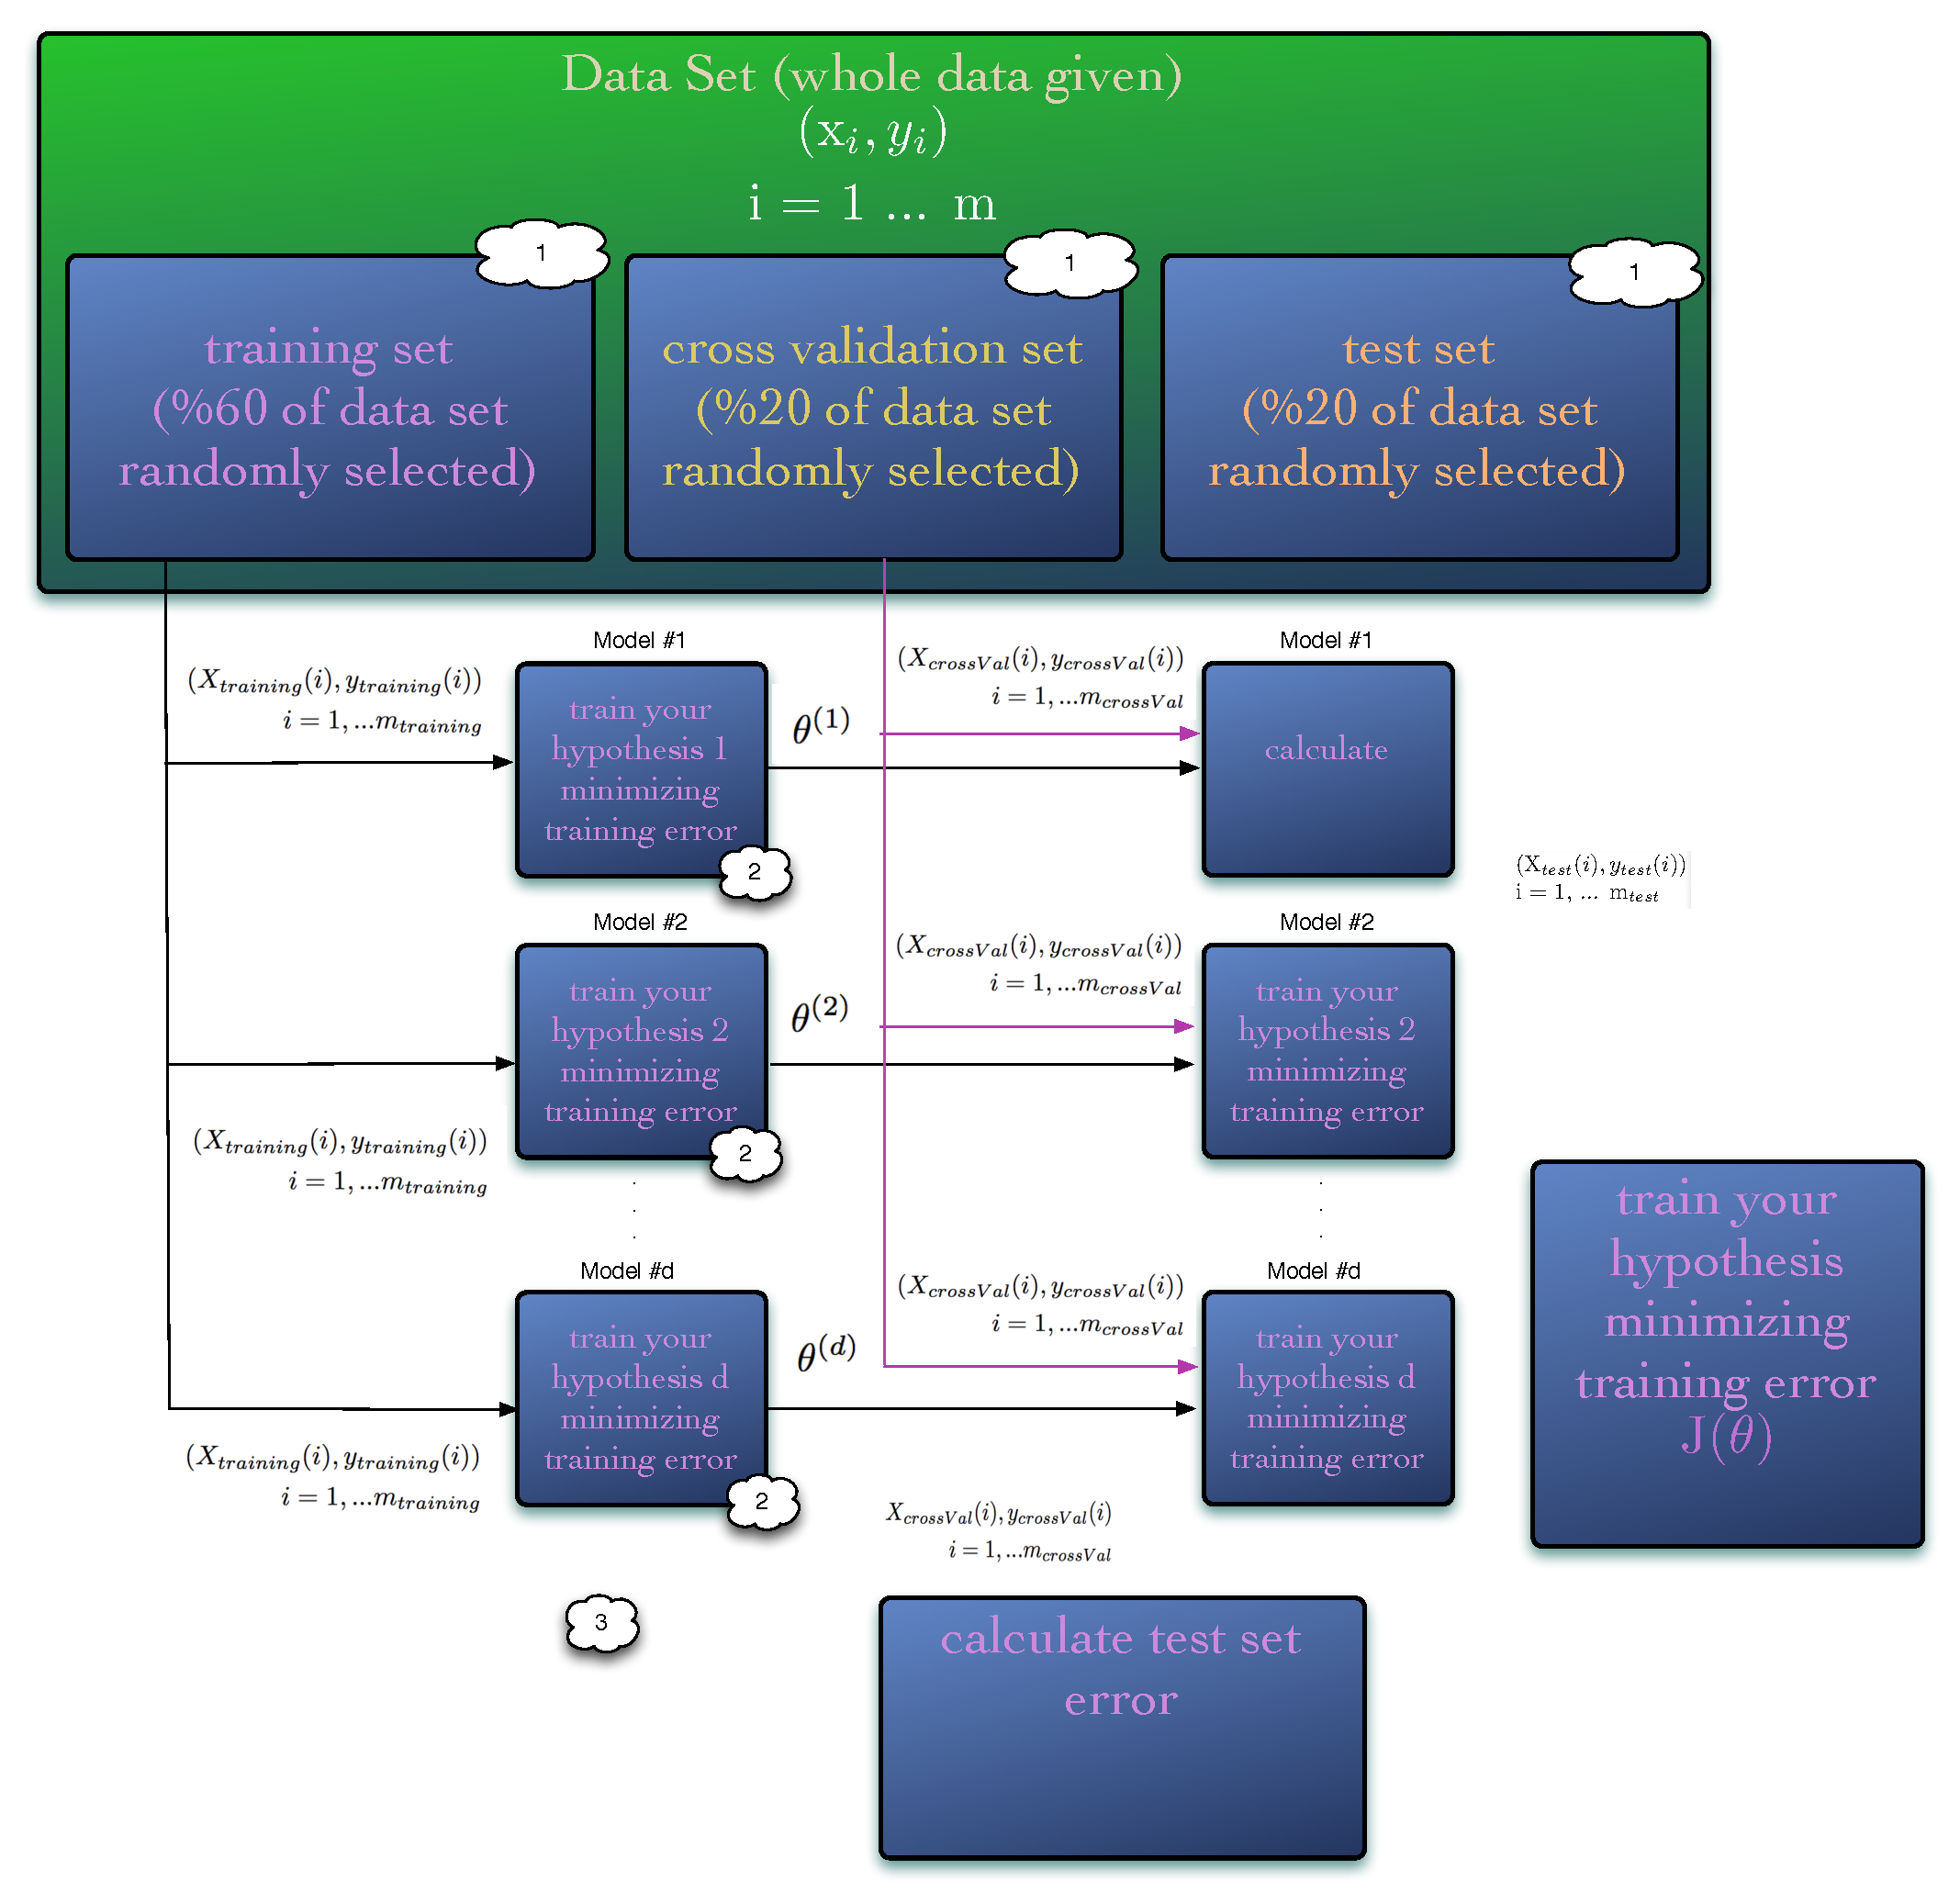
\includegraphics[width=16cm]{figures/modelSelection}    % The printed column width is 8.4 cm.
\includegraphics[width=23cm]{figures/modelSelectionNonVisualizableData}    % The printed column width is 8.4 cm.
\caption{Model selection guide} 
\label{fig:modelSelection}
\end{center}
\end{figure}
\end{landscape}
 
 \subsubsection{Normalization (Scaling)}

The next step is to normalize the data in order to constrain the values of feature change to within the same order of magnitude. 
This helps to improve the convergence rate of the optimization algorithm during the calculation of the model parameters $\bm{\theta}$.  
Although there are different methods for normalization, a common way is to use the formula:

\begin{equation}{\label{eqn:scalingFeatures}}
\bar{x}_j = \frac{x_j - \mu_j}{s_j} 
\end{equation} 

where the mean $\mu_j$ and range $s_j$ are given by

\begin{align}
\label{eqn:meandAndRange}
\begin{split}
\mu_j & = \frac{\sum\limits_{i=1}^m {x_j^i} }{m}
\\
s_j & = max(x_j) - min(x_j)
\end{split}
\end{align}

An important point is to keep that values $\mu_j$ and $s_j$ (or standard deviation in the cases it is preferred instead of range $s_j$) which are calculated during training. 
Those values are saved since they will also be used to scale the new inputs during the prediction phase.


\subsubsection{Training and evaluation of the classifier}  % Other subheadings have an inconsistent capitalization style

Here, it is assumed that we have selected one model and train the parameters of only this selected model. 
If multiple models are going to be evaluated, this training phase will be applied to all different models. 
Then, the selection of the best model should be done as already explained under \emph{Selecting the model} section.  

Before the training phase, the data should be split into two parts: training and test sets.
Then, the parameters $\bm{\theta}$ are learnt using the training data. 
Finally, the trained classifier is evaluated by calculating the test set error using the test set.
Those steps are given in more detail as follows:
 
 \begin{enumerate}
 
  \item Split the data set to two parts (30\% for the test set; 70\% for the training set). 
  Note that if the data set is randomly ordered, the first 70\% can be used for training and the rest for testing, but if the data is not randomly ordered (data is time dependent or if there is any correlation), the percentage of the data set for traing should be randomly selected between 30\% and 70\%. % Maybe check if I understood what you wanted to say!!
  
  \item Allow the model to learn the parameters $\bm{\theta}$ from the new training set (70\% of the whole data set). This step is further explained under \emph{Calculating parameters ${\bm{\theta}}$} section.

  \item Calculate the test set error by using the test set (30\% of all data) with the parameters learnt by using the training set (70\% of all data).\\
  For linear regression, the test set error is the cost function evaluated by the test set $(x_{test}(i), y_{test}(i))$ pairs and the parameters trained by using the training set $(x_{train}(i), y_{train}(i))$ and can be given as
	
	\begin{equation}{\label{eqn:costFuncTest}}
	J_{test}({\bm{\theta}})
	=\,
	\frac{1}{2m_{test}} \sum\limits_{i=1}^{m_{test}} \Big(h_{\bm{\theta}}(x_{test}^{(i)}) - (y_{test}^{(i)})\Big)^2  
	\end{equation} 
	
	For logistic regression, the test set error is given as
	
	\begin{equation}{\label{eqn:costFuncLogisticRegressionModified}}
	J_{test}({\bm{\theta}})
	=\,
	-\frac{1}{m_{test}} \sum\limits_{i=1}^{m_{test}} \Big[y_{test}^{(i)}\,log(\ h_{\bm{\theta}}(\ x_{test}^{(i)})) + (1-(y_{test}^{(i)}))\,log(\ h_{\bm{\theta}}(\ x_{test}^{(i)}))\Big]
	\end{equation} 
	
	Sometimes misclassification error (between 0 and 1), given in \ref{eqn:errorMisclassificationError}, is used instead of \ref{eqn:costFuncLogisticRegressionModified}
	% 0/1 misclassification error -> between 0 and 1 ... did I understand that right?

	\begin{equation}{\label{eqn:errorMisclassificationError}}
	 test\ error
	=\,
	\frac{1}{m_{test}} \sum\limits_{i=1}^{m_{test}} \Big(err(\ h_{\bm{\theta}}(\ x_{test}^{(i)}), (y_{test}^{(i)})\Big)  
	\end{equation}
	
	where the error function is given as

	\begin{equation}{\label{eqn:misclassificationError}}
	  err(h_{theta}(x),y)=\begin{cases}
               1 \qquad if\ h_{{\bm{\theta}}}\geq0.5,\ y=0 \ or\ if \ h_{{\bm{\theta}}} < 0.5, \ y=1\\
               0 \qquad otherwise\\
            \end{cases}
	\end{equation} 

\end{enumerate}

Fig.~\ref{fig:trainingAndEvaluation} visualizes and summarizes the procedure explained above.

\subsubsection{Calculating parameters $\bm{\theta}$}

The cost function is minimized to calculate the best $\bm{\theta}$ with the use of optimization algorithms. To fit the parameters $\bm{\theta}$, we will try to find those that minimize the cost function $J({\bm{\theta}})$

\begin{equation}{\label{eqn:optimizationGoal}}
\underaccent{{\displaystyle \bm{\theta}}}{min} \ J(\bm{\theta})
\end{equation} 

For the case of a simplified example with one feature, the minimization problem can be written as

\begin{equation}{\label{eqn:optimizationGoalSimplified}}
\underaccent{{\displaystyle \theta_0, \theta_1}}{min} \ J(\theta_0,\theta_1)
\end{equation} 

To achieve this minimization problem, there are a variety of algorithms available. 
A classical approach is the gradient descent method.  
Others include but are not limited to, conjugate gradient, BFGS (Broyden-Fletcher-Goldfarb-Shannon) algorithm, and L-BFGS (Limited-memory BFGS). 
They usually require the cost function, its gradient and the Hessian approximation in order to calculate the best $\bm{\theta}$ values.

\textbf{Gradient Descent}

Gradient descent will be presented for one feature problem due to its simplicity. 
Here, a linear regression problem is considered, where its hypothesis (model) and cost function is given in Equ.~\ref{eqn:linearRegressionTwoFeaturesSummary}

\begin{align}
\label{eqn:linearRegressionTwoFeaturesSummary}
\begin{split}
h_{{\bm{\theta}}}(x) & = \theta_0 + \theta_1 x_1 
\\
J(\theta_1,\theta_2)
 & =\,
\frac{1}{2m} \sum\limits_{i=1}^{m} \Big(h_{\bm{\theta}}(x^{(i)}) - (y^{(i)})\Big)^2  
\end{split}
\end{align}


\begin{landscape}
\begin{figure}
\begin{center}
\includegraphics[width=18cm]{figures/overfittingRealization}    % The printed column width is 8.4 cm.
\caption{Training and evaluating the classifier} 
\label{fig:trainingAndEvaluation}
\end{center}
\end{figure}
\end{landscape}



%\clearpage

The gradient descent algorithm for one feature is given as 

 \begin{algorithm}
   \caption{Gradient Descent for one feature only}
    \begin{algorithmic}[1]
      \Function{GradDesOneFeat}{$X, y, theta\_init, alpha, num\_iters$}       
      
      \Comment{Inputs: X - training inputs, y - training outputs, theta - parameters,\\ alpha - learning rate, num\_iters - 		number of iterations(termination condition)}

        \State $theta0 = theta(1))$  
        \State $theta1 = theta(2))$  
        \State $m = length(y)$ \Comment Number of training examples
%        \State Let $L[1 \ldots {n_1} + 1]$ and $R[1 \ldots {n_2} + 1]$ be new arrays

        \For{$j = 1$ to ${iter\_num}$} \Comment Do until satisfied
                \For{$j = 1$ to ${m}$}     \Comment Do for all training examples
                         \State initialize each grad to zero
           	 	\State $grad0 \leftarrow grad0 + (costFunc(x) - y)$
		         \State $grad1 \leftarrow grad1 + (costFunc(x) - y) * x$
                    \EndFor
                    \State $theta0 \leftarrow theta0 - alpha * grad0$
                    \State $theta1 \leftarrow theta1 - alpha * grad1$
        \EndFor
       \EndFunction

\end{algorithmic}
\end{algorithm}
 
A conventional approach to assign an initial value to ${\bm{\theta}}$ is to set $\theta_{init} = 0$.
It is important to know that for different initial values, ${\bm{\theta}}$ might converge to different values (local minima but not the global one) as in Fig.~\ref{fig:localOrGlobalMinimaGD}. 
But for linear regression, it is shown that the cost function shown above is convex, meaning that it has only one global minima with no other local minima. An example of the cost function converging to different solutions depending on initialization is given in Fig.\ref{fig:localOrGlobalMinimaGD} (a slightly different choice of $\theta_{init}$ might lead to a convergence to the local minima, where $J(\bm{\theta})$ is smaller compared to local changes in $\bm{\theta}$, but $J(\bm{\theta})$ is still not at its global minimum).

\begin{figure}
\begin{center}
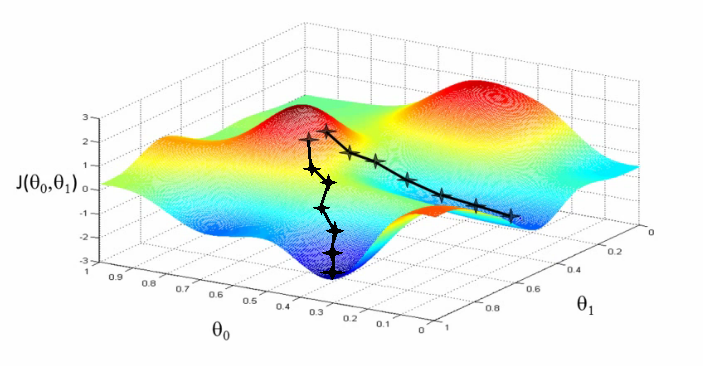
\includegraphics[width=11cm]{figures/localOrGlobalMinimaGD}    % The printed column width is 8.4 cm.
\caption{Gradient descent convergence dependance on $\theta_{init}$. Two different but close choice of $\theta_{init}$ might converge to local or global minima \cite{andrewNg_MachLearning}} 
\label{fig:localOrGlobalMinimaGD}
\end{center}
\end{figure}
 
Learning rate,  $\alpha$, gives the gradient descent its step size, so a larger value means a faster convergence. 
But keep in mind that for a larger alpha, the solution might not converge or even diverge, while too small values might lead the optimization to converge very slowly.
A set of $\alpha$ should be tried and evaluated by their performances. 
%A usual set to choose from would be $\alpha = [0.001, 0.01, 0.1, 0.003, 0.03, 0.3]$.
 Armigo-Goldstein rule can be used to set $\alpha$. 
%Number of iterations, $num\_iter$ is also a parameter to be chosen. 
%As a start, conventionally it can be selected as $num\_iter = 1000$ and then, convergence of the cost function should be checked. 
%If it has not yet converged but decreasing, a larger value for $num\_iter$ should be selected.

An important point in the algorithm is to update the $\bm{\theta}$ simultaneously. 
So during one iteration, the same $\bm{\theta}$ values should be substituted into $h_\theta(x)$, in order to calculate the next values of $\theta_0, \theta_1$.
 
\iffalse
Convergence of gradient descent can be debugged by plotting the cost function as a function of iterations of the optimization.
In the preferred case, the cost function should decrease in each iteration, never increase, and should converge to a steady value at the end of the optimization algorithm. 
Fig.~\ref{fig:visualizeCostFunc} shows two poor and one successful optimizations by plotting the cost function versus iteration. 

\begin{figure}[hbt]
\begin{center}
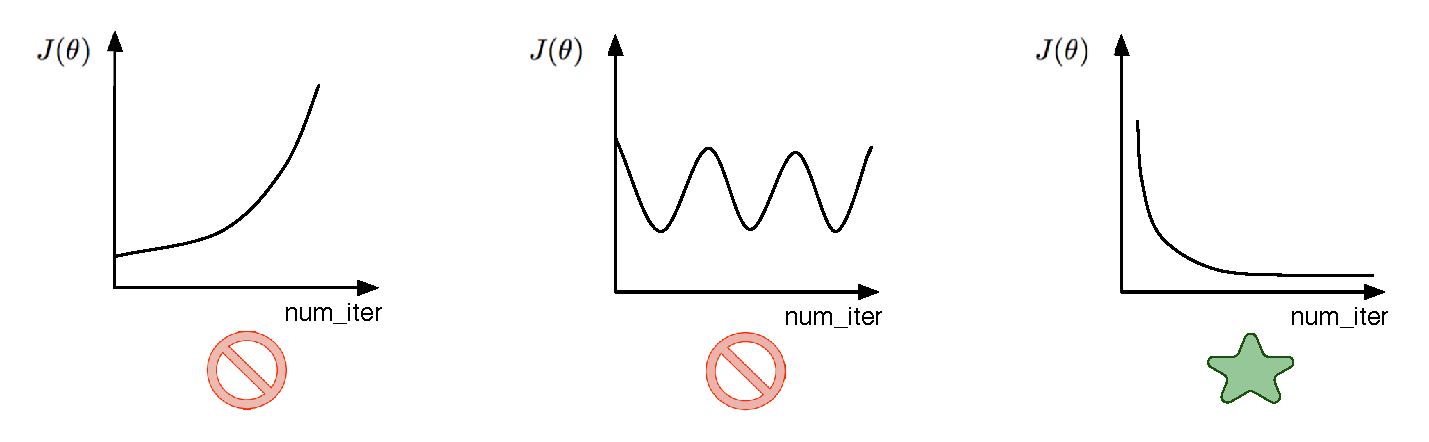
\includegraphics[width=15cm]{figures/visualizeCostFunc}    % The printed column width is 8.4 cm.
\caption{Evolution of $J(\theta)$ with respect to number of iterations. Left two figures showing that the optimization problem is not converging. The figure in the far right is the $J(\theta)$ evolution expected} 
\label{fig:visualizeCostFunc}
\end{center}
\end{figure}

Usually, it is a good practice to declare convergence when $J(\theta)$ decreases by less than $10^{-3}$ in one iteration. 
In case gradient descent is not converging, a smaller $\alpha$ should be tried. 
But too small values of $\alpha$ could result in a slow convergence. 

And finally, a generic gradient descent algorithm for multiple features can be given as below.

 \begin{algorithm}
   \caption{Gradient Descent}
    \begin{algorithmic}[1]
     \Function{GradDes}{$X, y, theta\_init, alpha, num\_iters$}    
           \State \textbf{Inputs:} X - training inputs, \\
           \qquad \qquad y - training outputs, \\
           \qquad \qquad theta\_init - initial guess for the optimized parameter theta,\\ 
           \qquad \qquad alpha - learning rate, \\
           \qquad \qquad num\_iters - number of iterations to find the optimized theta
           \State \textbf{Outputs:} theta - theta\_optimized/ theta vector that minimizes the cost function \\
           \qquad \qquad J - the values of the cost function calculated during the course of iterations
    \State repeat until convergence {
    \State $\theta_j \leftarrow \theta_j - \alpha \frac{\partial}{\partial \theta_j}J(\theta_0, \theta_1, \cdots)$
    	 \State For correct implementation, update simultaneously e.g
	 \State 	\qquad  $temp0 = \theta_0 - \alpha \frac{\partial}{\partial \theta_0}J(\theta_0, \theta_1, \cdots)$
	 \State 	\qquad  $temp1 = \theta_1 - \alpha \frac{\partial}{\partial \theta_1}J(\theta_0, \theta_1, \cdots)$
          \State 	\qquad  \qquad $\vdots$
          \State 	\qquad  $\theta_0 = temp0$
	 \State 	\qquad  $\theta_1 = temp1$
	 \State 	\qquad  \qquad $\vdots$
		 }
       \EndFunction
\end{algorithmic}
\end{algorithm}

\fi

\subsubsection{Overfitting}

Overfitting is common for complicated models or decision boundaries with high order polynomial terms such as

\begin{equation}{\label{eqn:featureMapping2}}
\bm{x_{mapped}}
=\,
\begin{bmatrix}
1 & x_1 & x_2 & x_1^2 & x_1x_2 & x_2^2 & x_1^3 \cdots & x_1x_2^5 & x_2^6 
\end{bmatrix}
\,^ T
\end{equation} 

If the model is suffering from overfitting, the trained model might end up fitting very well to the training set, but fail to generalize to the new data during the prediction phase. 
This means that the training set error is not a good predictor for how well the model would predict on new examples.

\begin{figure}[H]
\begin{center}
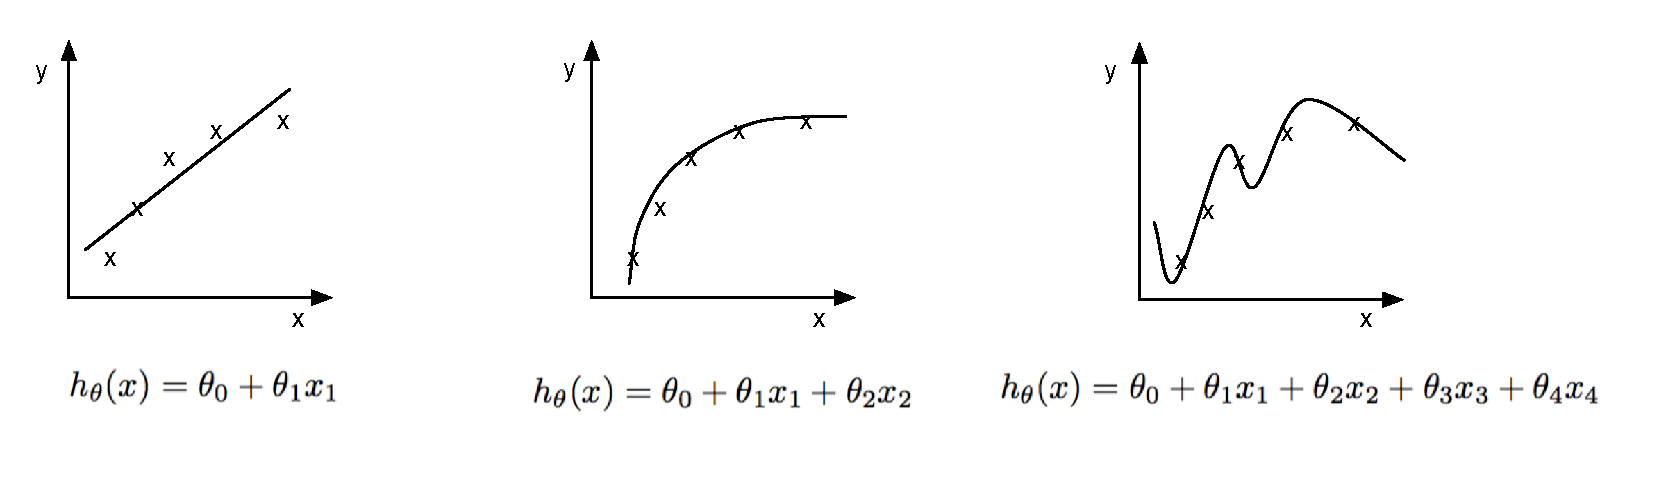
\includegraphics[width=16cm]{figures/underOverFit}    % The printed column width is 8.4 cm.
\caption{Underfitting, satisfactory or overfitting model examples (left to right)} 
\label{fig:underOverFit}
\end{center}
\end{figure}

Fig.~\ref{fig:underOverFit} shows three model examples plotted with the data that they are trained with. From left to right, those three regression problem models are underfitted, satisfactory or overfitted. 
But for problems with more features it might not be that obvious. Sometimes it might not even be possible to plot the model to realize if it is overfit or not.
For such cases, methods to detect overfitting should be used. 
To avoid overfitting, regularization parameter is used as explained in the next section.

\textbf{Regularization}

Regularization is practiced to avoid overfitting.
In regularization, a term is added to the cost function in order to penalize parameters $\vec{\bm{\theta}}$ for being too large (i.e to make $\vec{\bm{\theta}}$ as small as possible), except ${\theta}_0$ (is not penalized by convention). The cost function for linear regression with the added term for regularization is given as

\begin{equation}{\label{eqn:costFuncRegularized}}
J(\theta)
=\,
\frac{1}{2m} \bigg[ \sum\limits_{i=1}^{m} \Big(h_\theta(x^{(i)}) - (y^{(i)})\Big)^2 +\lambda \sum\limits_{j=1}^{n} \theta_j^2 \bigg] 
\end{equation} 

For logistic regression the regularized cost function can be written as (for two-class e.g $y \in \{0,1\}$)

\begin{equation}{\label{eqn:costFuncLogisticRegression}}
J(\theta)
=\,
\frac{1}{m} \sum\limits_{i=1}^{m} \Big[-y^{(i)}log(h_\theta(x^{(i)})) - (1-(y^{(i)}))log(1-h_\theta(x^{(i)}))\Big] +\frac{\lambda}{2m} \sum\limits_{j=1}^{n} \theta_j^2
\end{equation} 

Here, the challenge is to find the appropriate value for $\lambda$ which serves like a weight between the original part of the cost function and the second part, which penalizes $\bm{\theta}$ for being too large. 
So it tends to decrease the values of $\theta$. But if this lambda is too large, then the model converges to  

\begin{equation}{\label{eqn:costFuncRegularizedTooMuch}}
h_\theta(x)
=\,
\theta_0 
\end{equation} 

since all terms are penalized except $\theta_0$ (which is not penalized by convention) such that

\begin{equation}{\label{eqn:costFuncRegularizedTooMuchHow}}
h_\theta(x)
=\,
\theta_0 + \xcancel{\theta_1 x}  + \xcancel{\theta_2 x^2}  + \xcancel{\theta_2 x^3}  + \cdots + \xcancel{\theta_n x^n}
\end{equation} 

Thus, the model becomes underfitted for large values of $\lambda$, and it should be tuned to acquire the optimal value.


\subsubsection{Visualizing error to diagnose over-fit/under-fit problems}

To further debug the model, a guide is given in Fig.~\ref{fig:debuggingHypothesis}. 
Here, the errors for training and cross validation sets have to be calculated for a variety of polynomial degrees or regularization parameters. 
When training and cross-validation errors are plotted as a function of polynomial degree (or complexity of model), a larger training and cross-validation error shows that the model is likely to be an under-fit (high bias) model.  % MG: I thought the overfitted models were the ones with the higher biases - but maybe I misunderstood
A large cross-validation and low training error shows that the model is likely to be an over-fit model (high variance). 
Training and cross validation errors are calculated as in Equ.~\ref{eqn:costFuncTraining} and Equ.~\ref{eqn:costFuncCrossVal}. 
Here, it is assumed that there is no regularization term in the cost function. 
The training and cross validation errors are calculated in the same way as the cost function since the cost function itself is a measure of error.


\iffalse
\begin{equation}{\label{eqn:trainingError}}
J_{training}(\theta)
=\,
\frac{1}{2m} \sum\limits_{i=1}^{m} \Big(h_\theta(x^{(i)}) - y^{(i)}\Big)^2  
\end{equation} 

\begin{equation}{\label{eqn:crossvalError}}
J_{cv}(\theta)
=\,
\frac{1}{2m_{cv}} \sum\limits_{i=1}^{m_{cv}} \Big(h_\theta(x_{cv}^{(i)}) - (y_{cv}^{(i)})\Big)^2  
\end{equation} 
\fi

In the case that the cost function is regularized as given in Equ.~\ref{eqn:costFuncRegularized}, the training and cross validation errors are calculated ignoring the regularization term so they are defined exactly the same as given in Eq. \ref{eqn:costFuncTraining} and Eq. \ref{eqn:costFuncCrossVal} respectively.


Another way to diagnose learning problems is to plot training and cross validation errors with respect to training set size, also named as the learning curves (2 rightmost curves in Fig.~\ref{fig:debuggingHypothesis}). 
Although the training set size is normally constant, here we artificially reduce the number of training examples and calculate the training and cross validation errors. 
For that, the model parameters $\bm{\theta}$ are fit to this reduced training set and then the training and cross validation errors are also calculated over this reduced training data set. 
For the cases where the resulting curves give a low training error and a high cross validation error for smaller training set sizes and also high training and cross validation errors for larger training sizes, the problem is most likely to be suffering from under-fit (high bias). 
Another signature of an under-fit problem is that the training and cross validation errors are similar in magnitude. 

\begin{landscape}
\begin{figure}
\begin{center}
%\includegraphics[width=20cm,angle=90,origin=c]{figures/debuggingHypothesis}    % The printed column width is 8.4 cm.
\includegraphics[width=22cm]{figures/debuggingHypothesis}    % The printed column width is 8.4 cm.
\caption{Diagnosing machine learning problem by plotting training and cross-validation errors} 
\label{fig:debuggingHypothesis}
\end{center}
\end{figure}
\end{landscape}

If the learning curves give a low training error and a high cross validation error for the smaller training set size, and also training error is increasing with training set size while cross validation error decreasing without leveling off, the problem is more likely to be suffering from overfitting (high variance). 
Another important signature of an over-fit model is that the training error will be less than the cross validation error and the difference in between would remain significant. 


\subsubsection{Best practices}

After diagnosing the problem as over-fit or under-fit, the following practices are helpful to know. 

To fix an under-fit model, it would help to try 

\begin{itemize}

\item{Adding features}
\item{Adding polynomial features}
\item{Decreasing the regularization term}

\end{itemize}

To fix an over-fit model, it would help to try 

\begin{itemize}

\item{Adding more training examples}
\item{Decreasing the number of features}
\item{Increasing the regularization term}

\end{itemize}

\subsubsection{Prediction}

Finally, for a new set of input data, the output can be predicted using the trained model/classifier. 
One point to remember is that if scaling applied to the training set, new data should be scaled as well before being fed to the model/classifier using the same mean and standard deviation values previously calculated from the training set. 
After that, $h(\theta)$ could be evaluated using optimized $\theta$ and a scaled new data set $x\_new\_scaled$. 
So $h_\theta(x\_new\_scaled)$ gives

\begin{equation}{\label{eqn:prediction}
h_{\theta}(x\_new\_scaled})
=\,
P\Big(y=1 \, | \, x; \, \theta \Big)
\end{equation} 


which is the probability that $y = 1$ given $x\_new\_scaled$ parametrized by $\bm{\theta}$. 
%But still it is important to keep in mind, some other learning methods, the output of the problem could differ, such as the output of an SVM (Support Vector Method) classifier would be directly the class label.


\section{Support Vector Machines}

\subsection{Introduction}

\iffalse Let $ E = \Big\{ \big( \vec{\bm{x}}_1, y_1 \big),\big( \vec{\bm{x}}_2, y_2, 
		\cdots, \big( \vec{\bm{x}}_m, y_m \big) \big) \Big\}$, 
		where $\vec{\bm{x}}_i \in {\rm I\!R}^n$ and $y_i \in \big\{0, 1\big\}$ 
		be a training example set. Assuming the training data linearly separable, 
\fi		

SVM is a relatively new approach for classification, offering promising generalization properties thanks to its foundations on the structural risk minimization principle while other classifiers (such as logistic regression) usually only minimize the empirical risk \cite{gunn1998support,yin2014study}. 
This advances the capacity of generalization even with a small number of instances by reducing the risk of overfitting with properly tuned parameters. 
It can be applied to nonlinear systems and problems offering a vast number of features. 
Since the problem is represented as a convex optimization problem, SVM avoids local minima, to which Neural Networks(NN) are inherently prone to.

The aim of SVM is to find an optimal hyperplane maximizing the margin, which is the distance in between the boundaries, by extending them until hitting the first data point as in Fig.~\ref{fig:svmHyperplane}. These data points that are closest to the hyperplane (decision boundary) are called the support vectors and are the representatives of the data sets to be used for the decision process. This helps to abruptly decrease the data to handle, enhancing the ability to cope with the curse of dimensionality and reducing the computational complexity.

\begin{figure}
\begin{center}
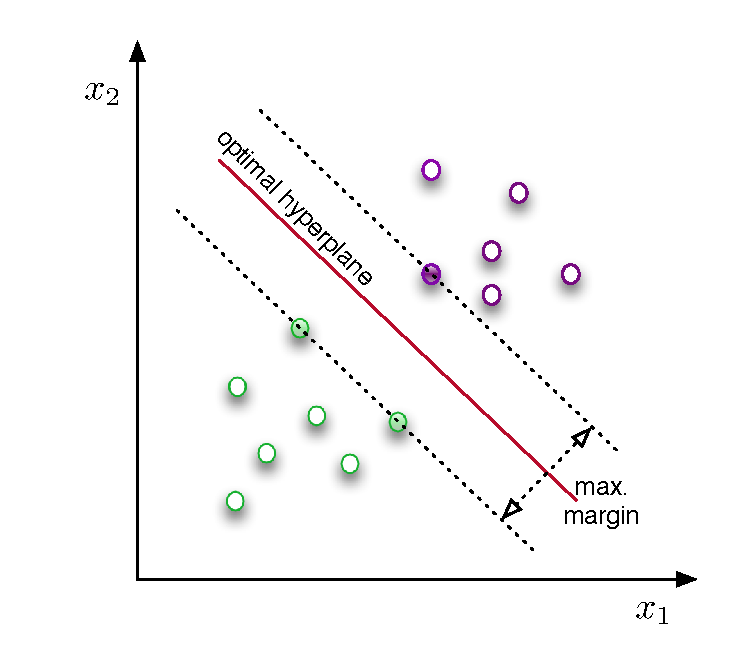
\includegraphics[width=9cm]{figures/svmHyperplane}    % The printed column width is 8.4 cm.
\caption{SVM working principle} 
\label{fig:svmHyperplane}
\end{center}
\end{figure}

SVM implements the idea of having a confidence in the prediction by using the concept of separating data with a large margin. 
Some other classification methods, such as logistic regression, output the probability of a new instance's belonging to a particular class, thus inherently give the confidence of the prediction as an output. 
On the other hand, SVM does only output if the new instance's probability of belonging to a particular class, so do not give its confidence on this decision explicitly. % This needs reformulating - I don't understand what you want to say here
Rather than including this confidence information as an output in terms of probabilities, this information is introduced with the functional and geometric margins. 
Methods are available for caluclating the posterior probabilities, which is the probability that the new measurements belongs to its predicted class\cite{platt1999probabilistic}. 
%An example of posterior probabilities showing new measurements' probabilities to belong to faulty class is given Fig.~\ref{fig:post_prob}. 

The training data set includes labeled data where the label can belong to one of two possible cases. This data set is saved in a matrix $\bm{X} \in {\rm I\!R^{m \times n}}  $ where $m,n$ correspond to number of instances and features respectively. The label information corresponding to the measurement instances is also fed to the SVM algorithm during the training phase as output vector $\bm{y} \in \{-1,1\}$. 

The aim of SVM is to find an optimal hyperplane maximizing the margin by solving the optimization problem for non-linearly separable datasets

\begin{align}
min_{\gamma,\omega,b} \quad & \frac{1}{2} \norm{\omega}^2 + C \sum\limits_{i = 1}^m \xi_i \\
s.t. \quad & y^{i}(\omega^T x^{(i)} + b) \geq 1 - \xi_i, \ i = 1, \cdots, m\\
 & \xi_i \geq 0, \ i = 1, \cdots, m
% hic bir sey yazmazsan esitlikleri alt alta hizaliyor canim benim&=alo \\
% $ tek dolar arasi $ inline denklem
% $$ cift dolar arasi $$ satir atlayarak ortada denklem
\end{align}

Here, the aim is to calculate the parameters $\omega$ and $b$ of the hypothesis by minimizing the objective function. In SVM, we drop the convention of denoting the hypothesis as $h(x)= \theta^T \, x$ and use $h_{\omega,b}(x)=g(\omega^T \, x + b)$ where $g(z) = 1$ if $z\geq0$ and $g(z)=-1$ otherwise. In order to generalize to the non-linearly separable datasets, $\xi_i$ is introduced in the equation's inequality constraint. Now, in the non-separable case, the functional margins ($y^{i}(\omega^T x^{(i)} + b)$) of the instances (examples) are permitted to have a value less than 1, different from when the case is separable. In order to ensure that most of the examples still do not violate the boundary, thus have a functional margin of at least 1, the objective function is also increased by $C \xi_i$. $C$ is called the box constraint, and usually needs to be tuned to achieve satisfactory performance.

Introducing the Lagrange duality to obtain the dual form of the optimization problem, use of kernels, to work efficiently in higher dimensional spaces, is eased. %I don't understand what you're trying to say in this sentence
The dual form also allows the use of efficient optimization solvers such as Sequential Minimal Optimization (SMO)  \cite{platt1998sequential}, which is the solver used in this work as well. Conventionally, the training phase of SVM requires the solution of a large quadratic programming (QP) problem. Especially for large training sets, computational heaviness of this phase might limit the applicability of SVM to specific problems sets. To overcome this constraint, SMO breaks the QP problem into a series of smaller QP problems which can be solved analytically. 

%Tolerance for the gradient difference between upper and lower violators obtained by Sequential Minimal Optimization (SMO) or Iterative Single Data Algorithm (ISDA), specified as the comma-separated pair consisting of 'DeltaGradientTolerance' and a nonnegative scalar.
% The default values are: 1e-3 if the solver is SMO (for example, you set 'Solver','SMO')

SVM has other tricks to deal with not linearly separable problems such as using kernels to map data into higher dimensional feature spaces where they can be separated with a linear hyperplane. Kernels are at the core of efficient SVM classifiers. A kernel, in general is defined as

\begin{equation}
K (x,z) = {\phi(x)}^T \phi(z)
\end{equation}

where $\phi$ represents the feature mapping. Usually the original features of the systems are named as attributes while the mapped set are called the features. In other words, $\phi$ maps the attributes to the features. Kernels offer various elegant properties such as computational efficiency. 
Cleverly selected, SVM classifiers can learn in high dimensional spaces represented by $\phi$ without the need to explicitly find or represent $\phi$, but instead calculating $K(x,z)$, which might be computationally more efficient. 

 
\subsection{Application}


A binary classifier is used in this work to classify two classes, faulty and nominal. 
SVM, being a supervised classification algorithm, has two main phases as shown in Fig.~\ref{fig:supervisedLearningBasics}: training and prediction. 


In the training phase, the model is taught to fit the labeled data that is fed to the SVM algorithm. The labeled data set is first divided into two portions with percentages of 80\% and 20\%, where the larger chunk is the training set and the remaining is the test set. 

This phase is usually followed with a tuning phase where some of the parameters of SVM are changed. Further, the training set is divided into cross-validation and training sets. The idea to split data is to avoid overfitting. When a model is overfit, it fits very accurately to the data it is trained with, but fails to generalize to new data. This results in a poor prediction performance. To avoid overfitting, which is the main problem of parametric discrimination approaches such as neural networks, parameter $C$ is tuned to result in an optimal fit with the cross validation set. Tuning $C$ also gives the user the ability to change the classifier's sensitivity to outliers, since sometimes finding a hyperplane separating all data perfectly is not the favorable option (this might cause overfitting). Then, the final performance of the classifier is tested on the test set. 

The classifier with the best performance is selected and then used in the prediction phase.  
For new data input, the classifier is used to predict which class the new data belongs to.



\subsubsection{Training of the classifier}

The first step is to normalize the features of the data as shown in Eq.~\ref{eqn:scalingFeatures} in order to make the values of features change within the same order of magnitude. 
Normalization offers advantages for the optimization algorithm and its convergence rate, during the calculation of model parameters.  
An important point is to keep the values of the mean and range $\mu_j, s_j$ (calculated with Eq.~\ref{eqn:meandAndRange}) and standard deviation (if it is used instead of range $s_j$). 
During the prediction phase, the data should first be scaled with these values attained from training data.

Default settings for SVM binary classification, included in Matlab Statistics and its Machine Learning Toolbox, utilizes SMO for optimization if outlier fractions are not specified during the function call. 

Default settings of Matlab's binary SVM classifier fits a linear model, which results in a linear decision boundary.  
In this study, a Gaussian Kernel, which corresponds to an infinite dimensional feature mapping, is used to map the attributes.

\begin{equation}
K (x,z) = exp \bigg(-\frac{\Vert x - z \Vert ^ 2}{2 \sigma^2} \bigg)
\end{equation}


\subsubsection{Tuning of the classifier}
% HIGH VARIANCE = OVERFIT =   LARGE C = SMALL sigma^2
% HIGH BIAS = UNDERFIT = SMALL C =  LARGE sigma^2
% sigma^2 LARGE = HIGH BIAS 

The training phase is usually followed by a tuning phase where some of the parameters of SVM are tuned and results are compared in order to have the best fit via cross validation set. This is the phase where the parameters of the classifier are fixed to be used in the last phase, prediction.

\begin{figure}
\begin{center}
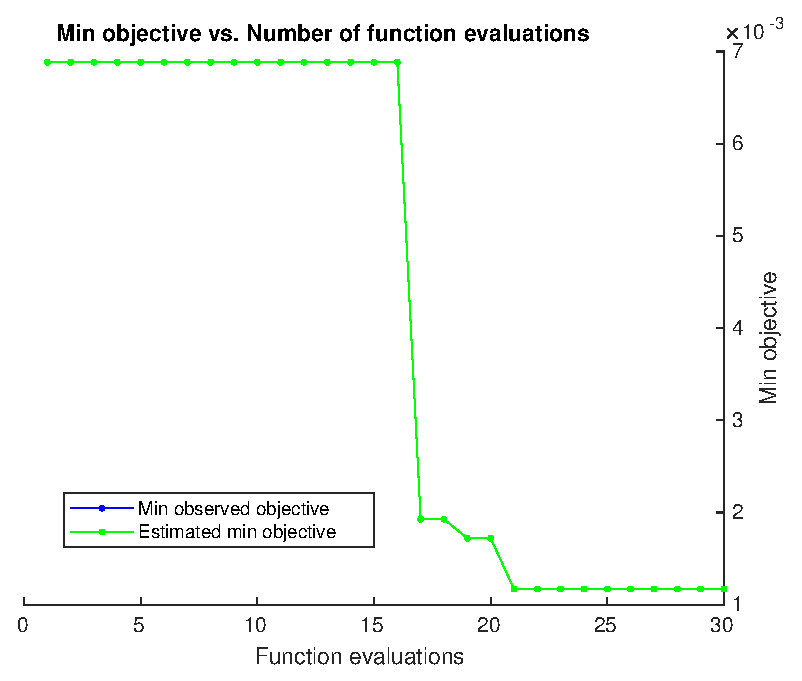
\includegraphics[width=0.7\textwidth]{figures/objectiveFuncEval}    % The printed column width is 8.4 cm.
\caption{Convergence of the objective function} 
\label{fig:objectiveFuncEval}
\end{center}
\end{figure}

To avoiding overfitting, which is the main problem of parametric discrimination approaches such as neural networks, $C$ (box constraint) and $\sigma$ (kernel scale), are tuned.
The classifier is trained with the training set and tuned via the cross validation set, and then the selected classifier is evaluated with the test set. The cross-validation set selection of Matlab uses a random selection over the data set. 
To compare different methodologies for tuning and also the untuned classifiers, the script has been revised to generate random values from the same seed value to be consistent in comparisons.
Box constraint ($C$) and kernel scale ($\sigma$) are tuned considering the presence of the outliers to generalize the distribution of the data rather than resulting in fine fits for each individual datum in the training set. 
% datum is singular of data

Two different ways are used to tune the classifier, heuristic and Bayesian optimization. In heuristic optimization, the strategy is to try a geometric sequence of the kernel scale (sigma parameter) scaled at the original kernel scale.  
Also box constraint parameters from a geometric sequence have been tried (11 values, from 1e-5 to 1e5 by a factor of 10). Increasing box constraint might decrease the number of support vectors, but also might increase the training time. 
Usually, increasing box constraint too much induces overfitting (high variance). 

\begin{figure}
\begin{center}
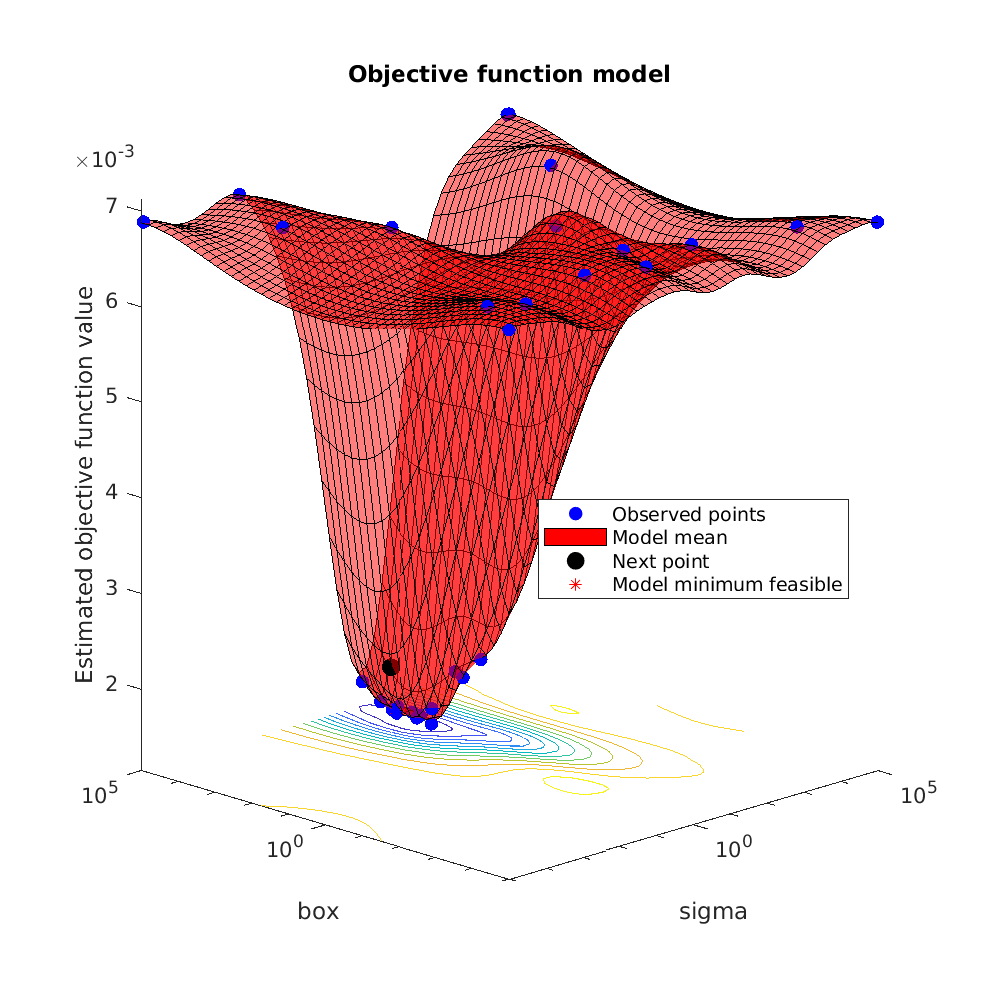
\includegraphics[width=0.7\textwidth]{figures/objFuncModel}    % The printed column width is 8.4 cm.
\caption{Objective function values for different box parameter and sigma values} 
\label{fig:objFuncModel}
\end{center}
\end{figure}


The Bayesian optimization tool from Matlab can be used in conjunction with the classification tool to optimize box constraint and the kernel scale. 
During the optimization, the objective function is printedwoth respect to function evaluations by the optimization tool as shown in Fig. ~\ref{fig:objectiveFuncEval}. Here, the objective is successfully converges to its minimum value after 21 function evaluations.
Fig. ~\ref{fig:objFuncModel} shows the objective function values for a variety of box constraint and kernel scale values. 
The optimized values for box constraint and kernel scale in each iteration are also presented as a table as given in Fig. ~\ref{fig:optBayesianSteps}. 
Also a summary of Bayesian optimization showing the calculated and estimated best values for sigma and box constraint is given at the end of optimization such as Fig. ~\ref{fig:optimBayesianResults}.
%After the training \& tuning is successfully completed, this model is used to predict the class of a new measurement. 

\begin{figure}
\begin{center}
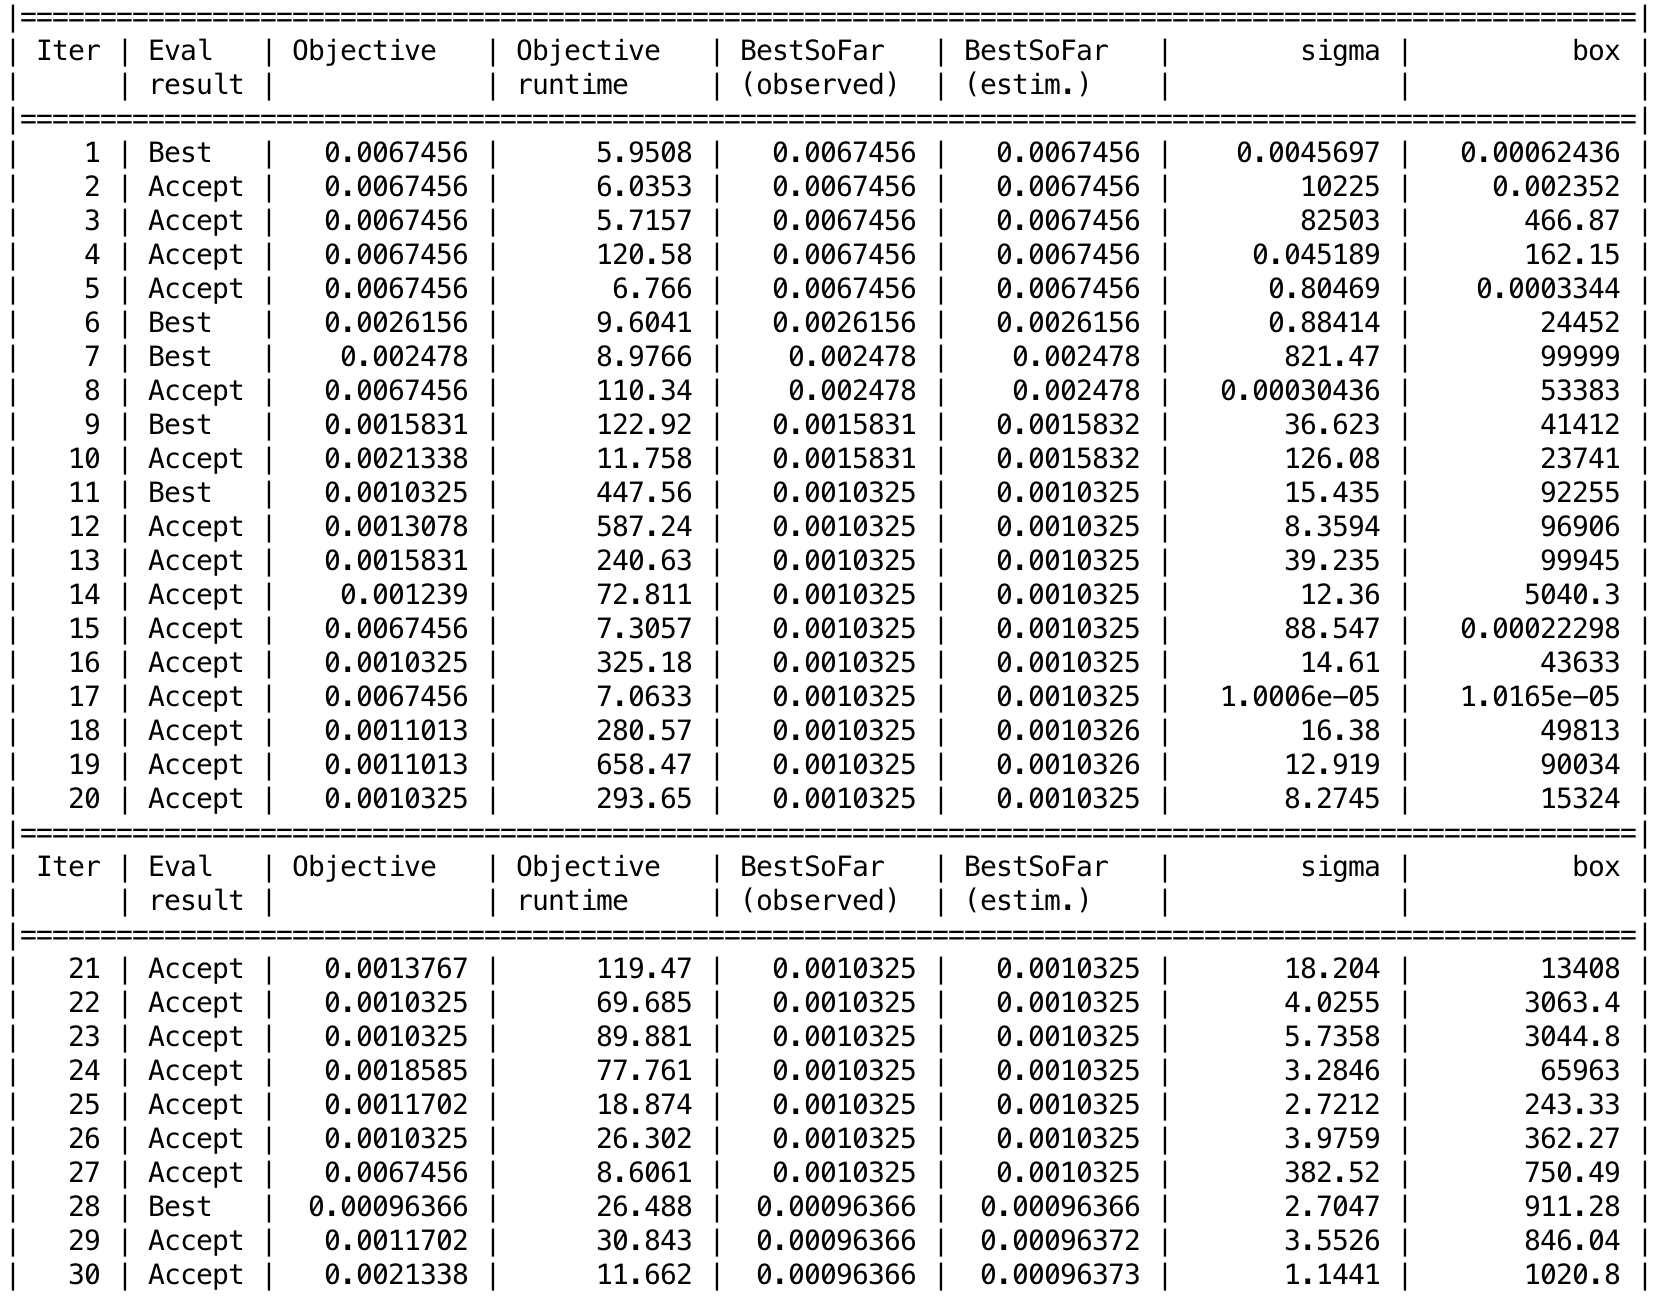
\includegraphics[width=1.13\textwidth]{figures/optimizationSummaryStuckFault}    % The printed column width is 8.4 cm.
\caption{Box constraint $C$, kernel scale $\sigma$ and objective function $J(\theta)$ values after each iteration during Bayesian Optimization. Minimum objective ($0.00096366$) can be seen at iteration number 28, and corresponding $C = 911.28$ (given as \emph{box}) and $\sigma = 2.7047$ (given as \emph{sigma}) are selected as the best values in this tuning.} 
\label{fig:optBayesianSteps}
\end{center}
\end{figure}

\begin{figure}
\begin{center}
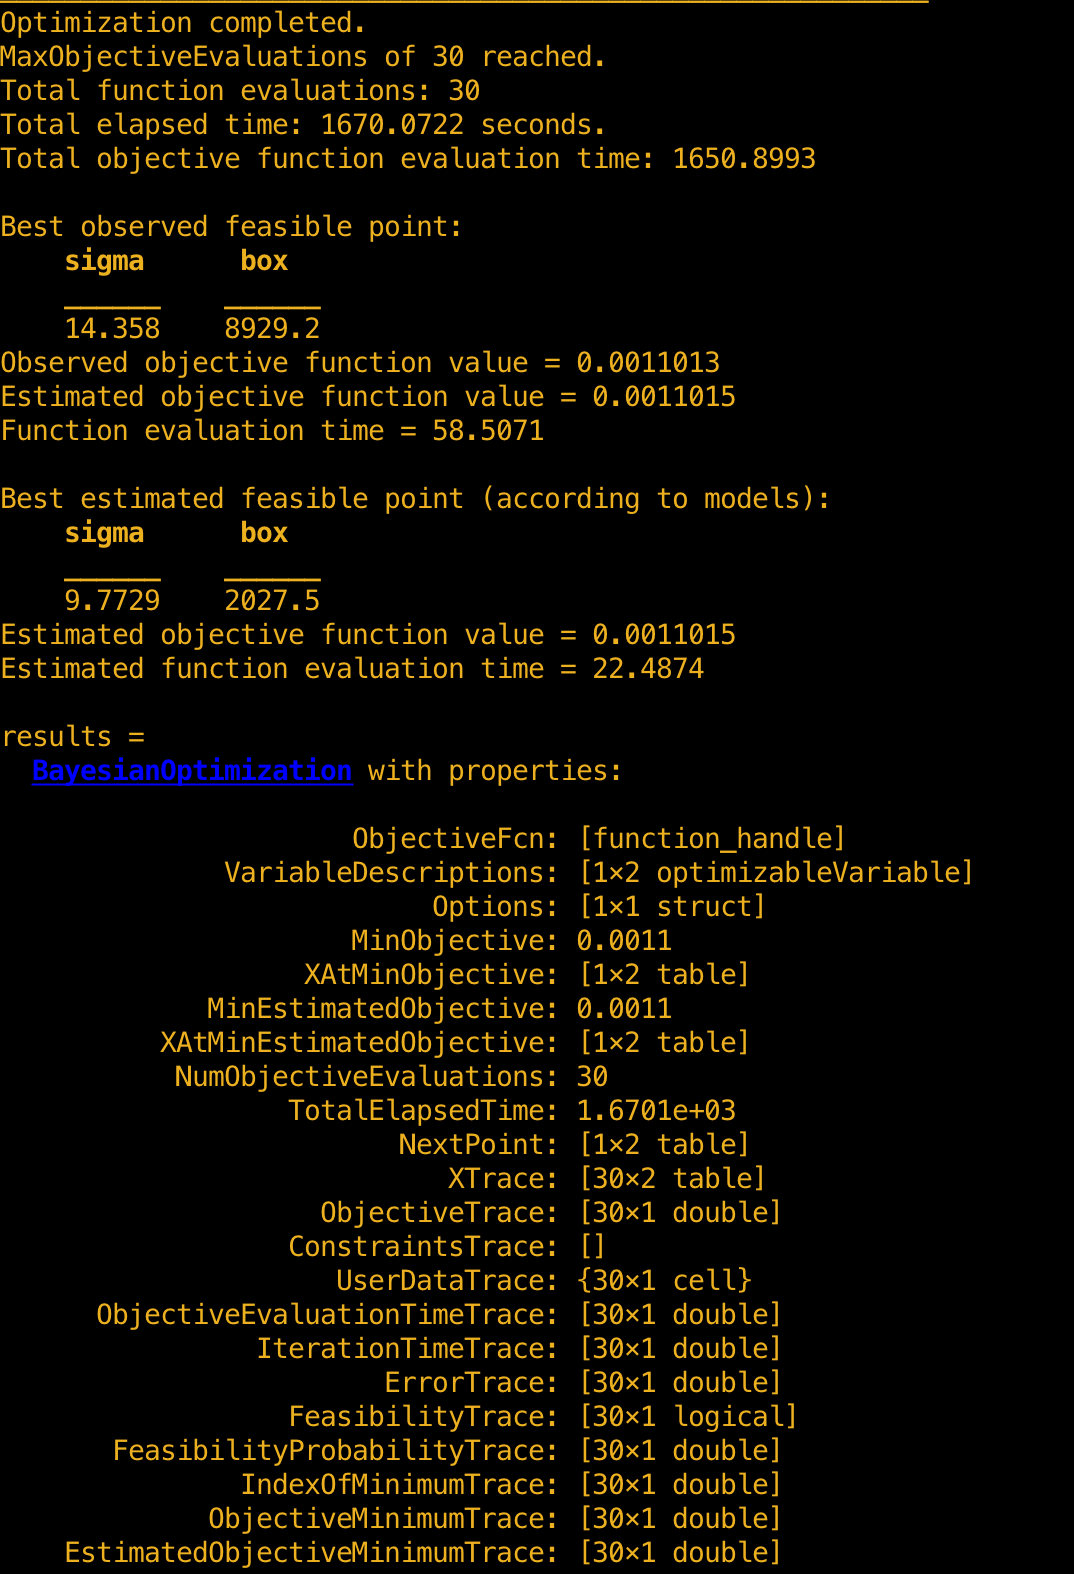
\includegraphics[width=0.6\textwidth]{figures/optimizationResultsStuckFault}    % The printed column width is 8.4 cm.
\caption{Final results for the optimization, time of execution, optimal values of box constraint and sigma values} 
\label{fig:optimBayesianResults}
\end{center}
\end{figure}

\subsubsection{Evaluating the classifier}
\label{evalClassifier}

The performance of the classifier is first quantified by \emph{loss of classification} (represented as \emph{kFoldLoss} in results) in this work. 
The training data set is separated into 10 folds. For each fold, the \emph{loss of classification} is computed for in-fold observations with a model trained on out-of-fold observations. 
Finally, taking an average of \emph{loss of classification} of 10 folds, final classification error is calculated.
The idea to split and evaluate the performance of classifiers on different data sets is to avoid overfitting since the fitted classifier would give better results on the data set that it learnt from, but might not generalize well to new data. 
%For that reason, both for evaluating the classifiers during tuning phase and finally evaluating the final classifier possessing the tuned parameters, were realized with different data sets.

Another means to evaluate performance of a classifier, available under Matlab Statistics and Machine Learning Toolbox, is via observing the \emph{classification edge}. 
The \emph{edge} is the weighted mean of the \emph{classification margins}. 
Here, the \emph{classification margin} for a binary classifier is defined, for each observation, as the difference between the \emph{classification score} for the \emph{true class} (faulty measurements in the considered problem) and the \emph{classification score} for the \emph{false class} (nominal measurements in the considered problem). 
In this definition, \emph{classification score} is considered as the signed distance from each observation to the decision boundary.

While all these variables would be satisfactory for performance analysis of classifiers, due to the skewed-class nature of the problem, another means of evaluations is necessary.
When the number of instances for different classes in a data set has a big difference, it is named as a skewed-class problem. 
The inherent trickiness to evaluate classifiers for such problems lies on the fact that, predicting only the more frequent class might lead to a misunderstanding that the classifier gives superior performance although it might not be even learning at all. 
For the problem of fault detection of a control surface would serve as a good example to clarify more. 
Since nominal data is not difficult to generate in real flight while it is difficult to fly faulty, the nominal data is much vast compared to the faulty data 

For such problems, in order to define a single metric to evaluate the abilities of classification, \emph{precision} and \emph{recall} should be defined.   
Fig.~\ref{fig:confusionMatrix} shows the confusion matrix which is used to calculate the precision and recall. 
Here, in general, the class indicated by 1 is the skewed class, corresponding to the fault class in this study. 
True positive refers to the number of instances that are predicted faulty and are actually faulty, false positive refers to the number of nominal instances which are miscalculated or predicted as faulty, false negative is the number of instances that are actually faulty but the classifier predicted that they are nominal, and finally the true negative is the number of instances that are predicted as nominal and are actually nominal.
Precision gives a measure on the fraction that was actually faulty of all the measurements that was predicted as faulty. 
Precision can be related to number of false alarms which is cautiously avoided in flight control systems. Precision is defined as 

\begin{figure}
\begin{center}
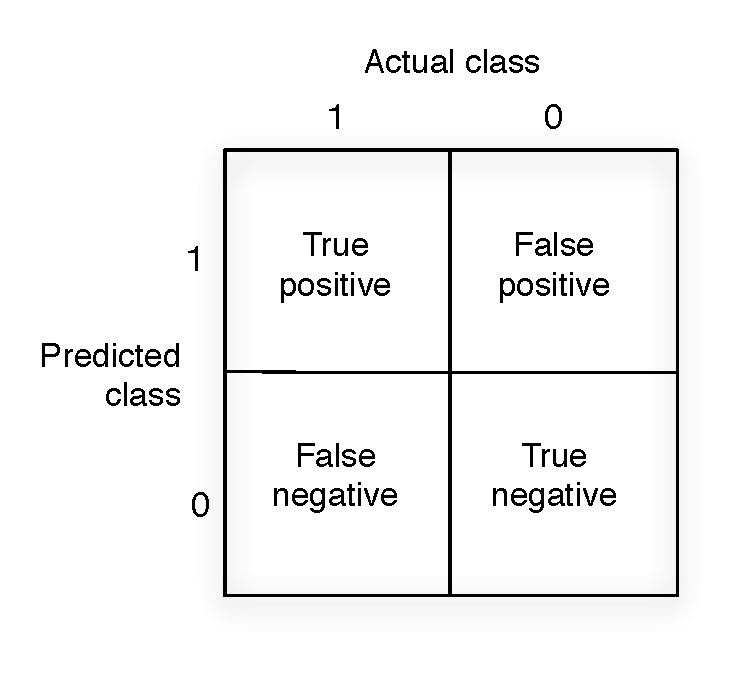
\includegraphics[width=0.5\textwidth]{figures/confusionMatrix}    % The printed column width is 8.4 cm.
\caption{Confusion matrix} 
\label{fig:confusionMatrix}
\end{center}
\end{figure}


\begin{equation}
precision = \frac{true \ positives}{true \ positives + false \ positives}
\end{equation}

Recall refers to the fraction of correctly detected faults of all the situations that were actually faulty. 
Recall can be related to the sensitivity of diagnostic systems. 
Actually an ideal health monitoring system is the one which accomplishes a reasonable balance between the false alarm rate and ability to detect reasonably small faults. 

\begin{equation}
recall = \frac{true \ positives}{true \ positives + false \ negatives}
\end{equation}

Finally as a single metric to evaluate the performance of the classification, F1 score is defined as

\begin{equation}
f1Score = \frac{2 * precision * recall}{precision + recall}
\end{equation}

F1 score, indicated as f1Score in the tables throughout this study is used as the main parameter to evaluate classifiers.

\section{Conclusion}
In this chapter, an introduction to machine learning algorithms is presented. 
Two main branches of machine learning, supervised and unsupervised learning are introduced. 
Terminology and construction of input and output vectors are presented using easy examples of regression and classification. 
Regression and classification are two common problems discussed under supervised learning problem. 
The problems that are frequently encountered during machine learning applications are discussed and best practices to achieve more accurate results are presented. 

After this generic introduction to machine learning implementations, \emph{Support Vector Machines} (SVM) are discussed.  
A very brief section explains their mathematical background and then application procedures are presented.

The next chapter will explain the simulation results by applying SVM to drone flight data. First, results from application of SVM to simulated measurements are presented. Then, SVM is applied to flight data. To be precise on how the data is generated, the injection of faults during flight and the modifications to the \emph{Paparazzi} autopilot in order to realize the faults are explained in detail.
